\documentclass[10pt, aspectratio=169]{beamer}
\PassOptionsToPackage{table,xcdraw}{xcolor}
\usepackage{graphicx}
\usepackage{amsmath}
\usepackage{subcaption}
\usepackage{media9}
\usepackage{multicol}
\usepackage{circuitikz}
\usepackage{tikz}
\usetikzlibrary{automata, positioning}
\usepackage{listings}
\usepackage{xcolor}
\usepackage{booktabs}

\usepackage{multirow}      % For merging rows in tables
\usepackage{colortbl}      % For coloring cells
\usepackage[table,xcdraw]{xcolor}  % For extended color options in tables

\usepackage{fqsstyle/beamerthemefqs}
\usepackage{fqsstyle/beamercolorthemefqs}

\usepackage{hyperref}
\hypersetup{
    colorlinks=false,
    % linkcolor=umBlue,
    % filecolor=magenta,
    % urlcolor=cyan,
    % pdftitle={Overleaf Example},
    % pdfpagemode=FullScreen,
    }
\usepackage{xcolor}
\usepackage{amsmath}
\usepackage{wrapfig}
\usepackage{graphicx}
\usepackage{helvet}
\usepackage[T1]{fontenc}
\usepackage{tikz}
\usetikzlibrary{shapes, arrows, calc, positioning, patterns}
\usetikzlibrary{decorations.pathreplacing}
\usepackage{amsmath,amssymb, amsfonts}
\usepackage{lipsum}
\usepackage{datetime}
\usepackage{setspace}
\usepackage{listings}
\usepackage{fancyvrb}
%%% Local Variables:
%%% mode: latex
%%% TeX-master: "../main"
%%% End:

\renewcommand{\familydefault}{\sfdefault}
\renewcommand\mathfamilydefault{}
\newcommand{\colorbf}[1]{{\color{umGreen}\textbf{#1}}}

\newdateformat{dmydate}{%
  \twodigit{\THEDAY}~\monthname[\THEMONTH] \THEYEAR%
}

%%%%%%%%%%%%%%%%%%%%%%%%%%%%%%%%%%%%
%% eqauation
%%
\DeclareMathAlphabet{\mathbfsf}{\encodingdefault}{\sfdefault}{bx}{n}
% \renewcommand{\vec}[1]{\mathbfsf{#1}}
\newcommand{\vect}[1]{\vec{\mathbf{#1}}}
\newcommand{\brak}[1]{\langle{#1}\rangle}
\newcommand{\rbrak}[1]{\left({#1}\right)}
\newcommand{\sbrak}[1]{\left[{#1}\right]}
\newcommand{\cbrak}[1]{\left\{{#1}\right\}}
\newcommand{\abrak}[1]{\left|{#1}\right|}
\newcommand{\intInf}{\int_{-\infty}^{+\infty}}
\newcommand{\intinf}{\int_{-\infty}^{\infty}}
\newcommand{\conj}{\mathlarger{*}}%
\newcommand{\Psiconj}{\Psi^\conj}
\newcommand{\Psixt}{\Psi\rbrak{x,t}}
\newcommand{\hi}{\hat{i}}
\newcommand{\hj}{\hat{j}}
\newcommand{\hk}{\hat{k}}
\newcommand{\hx}{\hat{i}}
\newcommand{\hy}{\hat{j}}
\newcommand{\hz}{\hat{k}}
\newcommand{\vB}{\vect{B}}
\newcommand{\vE}{\vect{E}}
\newcommand{\vD}{\vect{D}}
\newcommand{\vH}{\vect{H}}
\newcommand{\curl}[1]{\vect{\nabla}\times\vect{#1}}
\newcommand{\divg}[1]{\vect{\nabla}\cdot\vect{#1}}

% quote
\newcommand{\q}[1]{``#1''}

%%% Local Variables:
%%% mode: latex
%%% TeX-master: "../main"
%%% End:


%%% Local Variables:
%%% mode: latex
%%% TeX-master: "../main"
%%% End:


\mode<presentation>{%
    \usetheme{fqs}
    \usecolortheme{fqs}
}

\title[NeSy CER in Autonomous Driving]{Neuro-symbolic Complex Event Recognition in Autonomous Driving}
\subtitle[YABT]{MSc in Artificial Intelligence Thesis \\ @
NCSR Demokritos \& University of Piraeus}
\titlebackground{fqsstyle/assets/gambar-um.jpg}
\author{\textcolor{umBlueLighter}{Tatiana Boura} and \textcolor{umBlueLighter}{Nikos Katzouris}} % Your name
\institute[NCSR Demokritos]
{\noindent
    \textit{tatianabou@iit.demokritos.gr}\par
    \textit{nkatz@iit.demokritos.gr}\par
}

\date{03 October 2024} 

\setbeamersize{text margin left=.05\pdfpagewidth,text margin right=.05\pdfpagewidth}

\begin{document}

%%%%%%%%%%%%%%%%%%%%%%%%%%%%%%%%%%%%
%%  CUSTOM TITLE PAGE: with featured image
%%
{
  \setbeamertemplate{headline}{}
  \begin{frame}
      %%%%%%%%%%%%%%%%%%%%%%
      %% Featured Image (comment or delete if not used)
      %%
      \begin{tikzpicture}[overlay, remember picture]
          \node[left=1.0cm] at (current page.1){%
              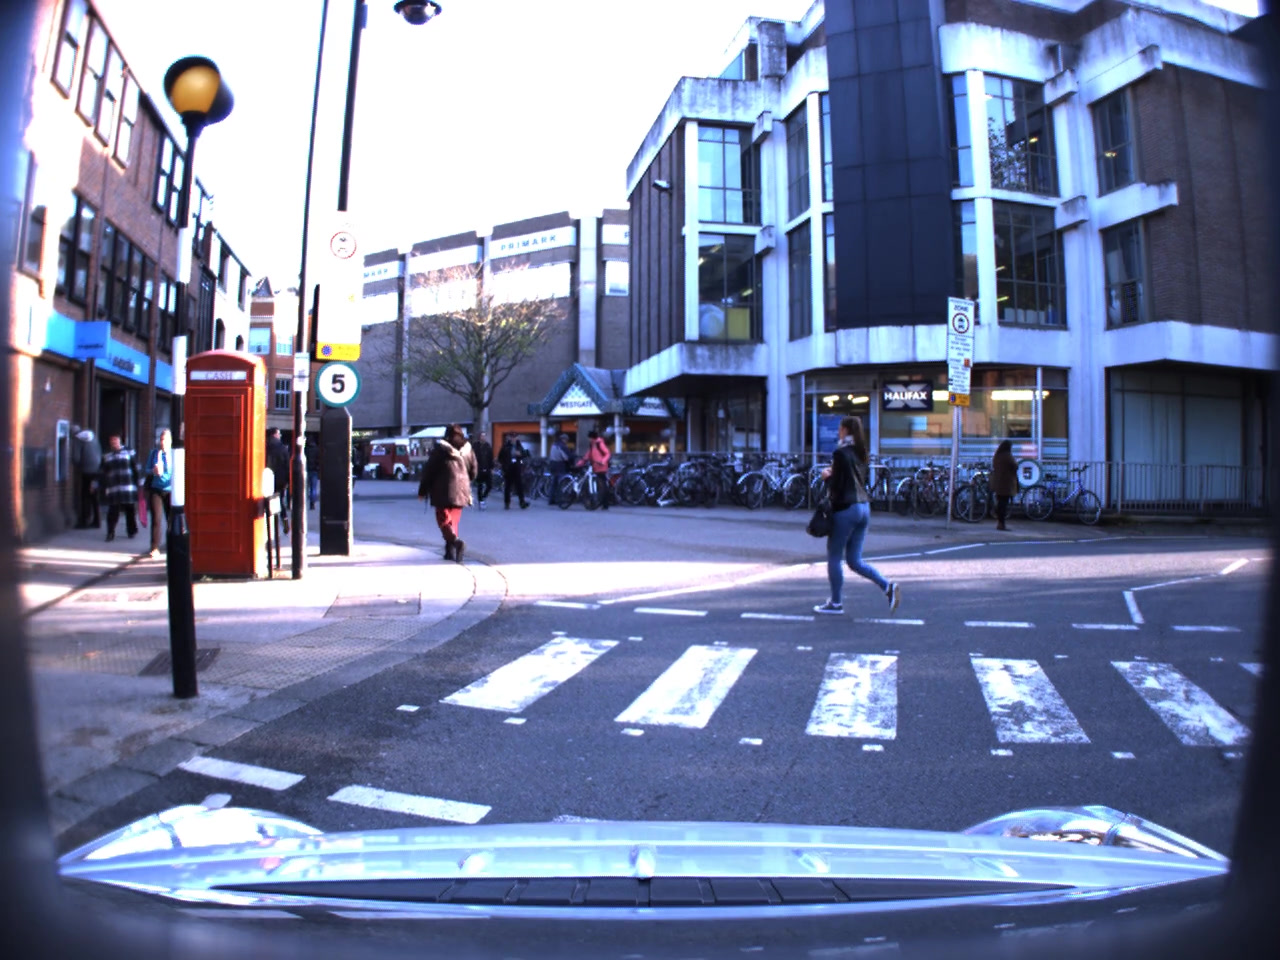
\includegraphics[width=6.5cm]{contents/images/00019.jpg}
          };
      \end{tikzpicture}
      % the title page itself
      \titlepage%
  \end{frame}
}

%%%%%%%%%%%%%%%%%%%%%%%%%%%%%%%%%%%%
%% SECTION PAGE: without background image
%%
\section{Introduction}
{
    \setbeamertemplate{headline}{}
    \begin{frame}
        \sectionpage%
        %%%%%%%%%%%%%%%%%%%%%%
        %% Featured Image
        %%
        \begin{tikzpicture}[overlay,remember picture]
            \node[left=2cm] at (current page.2){%
                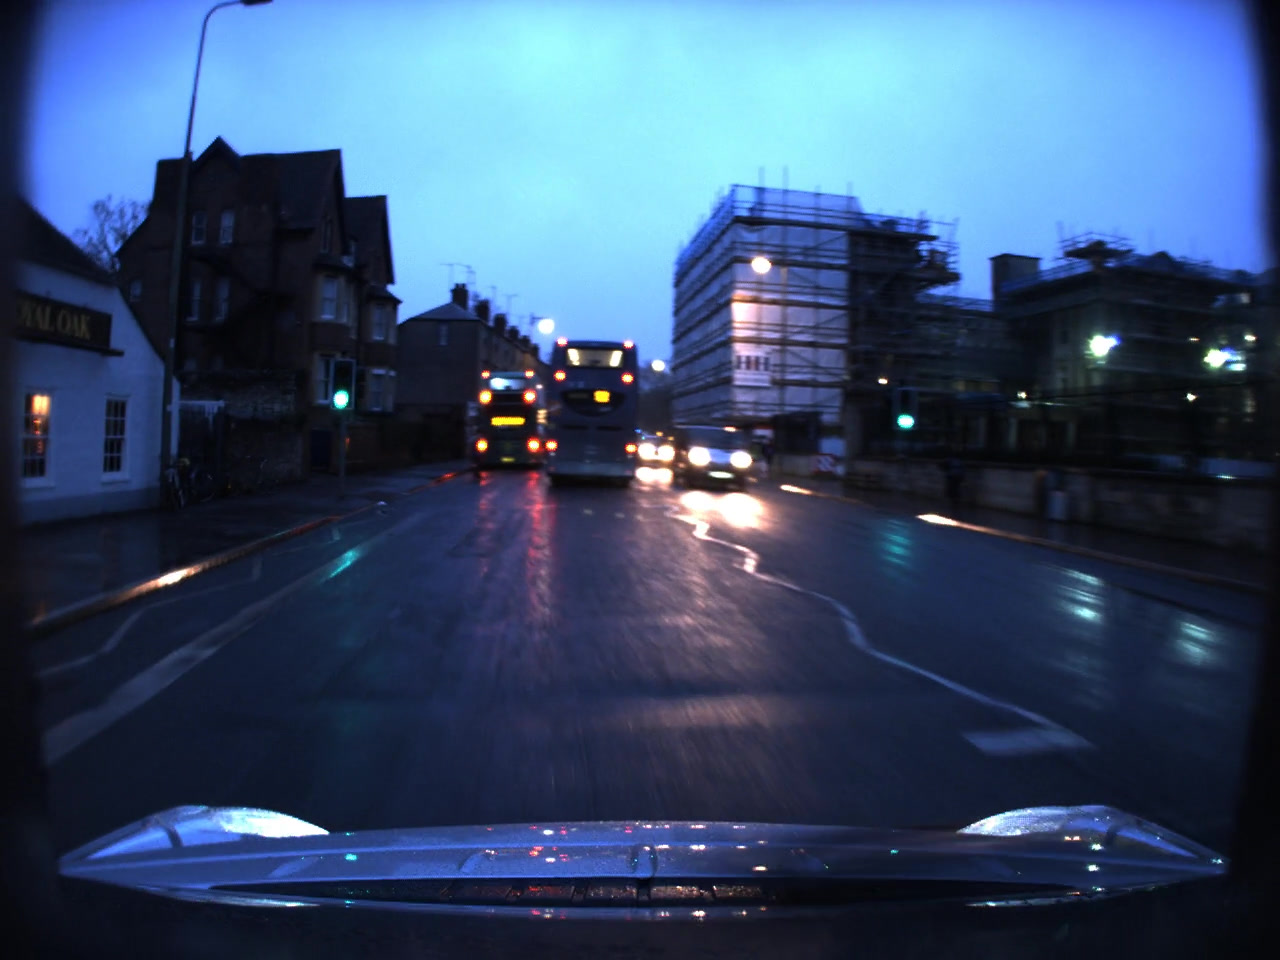
\includegraphics[width=5.5cm]{contents/images/01833.jpg}
            };
        \end{tikzpicture}
    \end{frame}
}

\begin{frame}{Introduction and Motivation}
% Very generally, we will converge as the time passes
    \begin{itemize}
        \setlength{\itemsep}{12pt}
        \item \textcolor{umBlueLighter}{Complex event recognition (CER)} involves efficiently identifying spatio (temporal) events within Big Data streams 
        \item CER systems use well-defined theoretical frameworks, such as (symbolic) automata
        \item In some case processing of \textbf{sub-symbolic streams} is required
        \item To enhance the systems' performance, \textcolor{umBlueLighter}{Neuro-Symbolic Artificial Intelligence (NeSy)} methods are being used
        \item In this work we introduce a NeSy CER framework which we evaluated on the autonomous driving domain
    \end{itemize}
\end{frame}

\section{Background}
{
    \setbeamertemplate{headline}{}
    \begin{frame}
        \sectionpage%
        %%%%%%%%%%%%%%%%%%%%%%
        %% Featured Image
        %%
        \begin{tikzpicture}[overlay,remember picture]
            \node[left=2cm] at (current page.2){%
                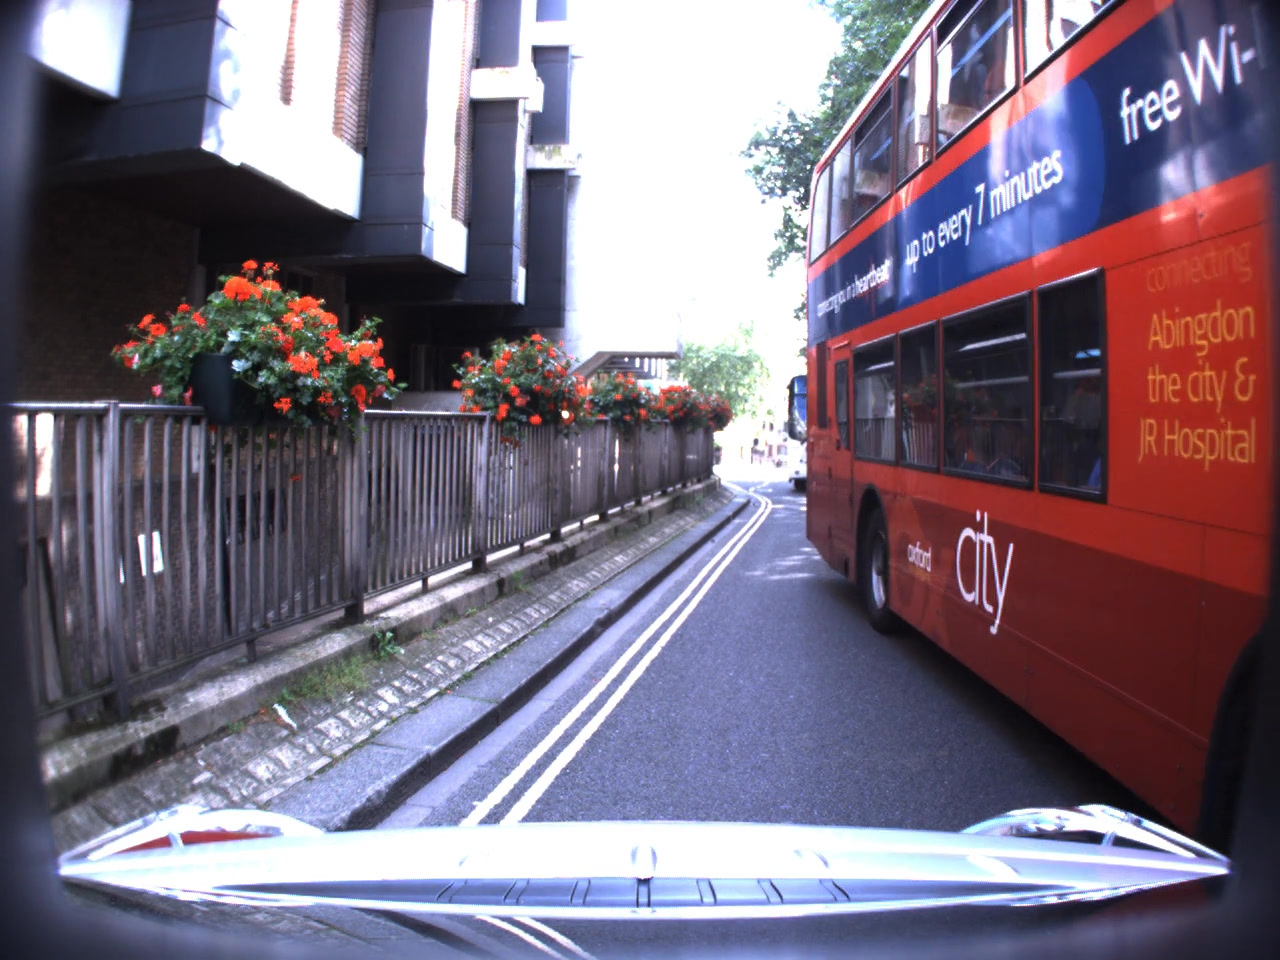
\includegraphics[width=5.5cm]{contents/images/04123.jpg}
            };
        \end{tikzpicture}
    \end{frame}
}

\begin{frame}{Complex Event Recognition (CER)}
    \begin{itemize}
        \setlength{\itemsep}{12pt}
        \item CER, or complex event pattern matching, refers to the process of detecting patterns in streams of continuously arriving timestamped `event' data from distributed sources
        \item \colorbf{Key Concept}: These \textcolor{umBlueLighter}{simple events} \textit{make up} \textcolor{umBlueLighter}{complex events}
        \item CER systems have strict time-response constraints and are expected to perform efficiently 
        \item What differentiates them from $\dots$
        \vspace{0.6em}
        \begin{itemize}
            \setlength{\itemsep}{4pt}
            \item \textbf{Traditional database systems? } Data-streams do not need to be stored
            \item \textbf{Classical stream querying?} The system has  the responsibility to interpret the result
        \end{itemize}
    \end{itemize}
\end{frame}

\begin{frame}{CER Systems and Languages}
    \begin{itemize}
        \setlength{\itemsep}{12pt}
        \item Logic-based (e.g.,\textit{event calculus}), tree-based and \textcolor{umBlueLighter}{automata based}
        \item Event streams are sequences of events $\rightarrow$ automata are common computational models for CER systems
            \vspace{0.6em}
            \begin{itemize}
            \setlength{\itemsep}{4pt}
                \item Patterns are typically defined in a declarative language and then translated into automata
                \item The automaton processes a stream of simple events, changing states when predicates on outgoing transitions from the current state are satisfied
                \item A complex event is detected whenever the stream reaches a \textbf{final state}
            \end{itemize}
    \end{itemize}
\end{frame}

\begin{frame}{CER in Autonomous Driving}
    \begin{itemize}
        \setlength{\itemsep}{12pt}
        \item Self-driving cars have been receiving attention for quite some time % money and vast research into this
        \item In literature tasks within the autonomous driving domain are not described in CER terms, but they \textit{can be}:  \\
        \vspace{0.6em}
        \begin{center}
         A \textbf{large volume} of sensor data must be processed \textbf{rapidly}, \textbf{efficiently}, and \textbf{robustly} to detect \textbf{events} following specific \textbf{sequences} of events (\textit{e.g., sudden braking}).
          \end{center}
        \item \textcolor{umBlueLighter}{Why CER?} Because $\dots$
        \vspace{0.6em}
            \begin{itemize}
            \setlength{\itemsep}{4pt}
                \item $\dots$ sometimes we want to use `known' patterns of an event
                \item $\dots$ when we learn patterns, we need them to be interpretable
            \end{itemize}
        \item We will focus on tasks that require deep vision % and not for example the robotics stuff
    \end{itemize}
\end{frame}

\begin{frame}{Motivation for the rest of the Background}
    \begin{itemize}
        \setlength{\itemsep}{12pt}
        \item CER systems handle \textbf{symbolic data}, %(human-readable representations of knowledge) 
        \textit{but} our goal is to perform it on \textbf{sub-symbolic} %(distributed, numerical representations less transparent to human understanding)
        \item So, we use NNs for the sub-symbolic video input (\textit{simple events}) and allow pattern matching (\textit{complex events}) to be handled by the symbolic part
        \item The challenge lies in the alignment of the NN with the automata (\textcolor{umBlueLighter}{NeSy integration})
        \item The alignment does not only refer to inference, but also \textbf{training} (distant supervision)
        \item For training the NN, the whole system needs to be differentiable
        \vspace{0.6em}
            \begin{itemize}
            \setlength{\itemsep}{4pt}
                \item \colorbf{How?}  Probabilistic inference
                \item \colorbf{Why?}  Differentiable circuits answer probabilistic queries (\textit{is it a complex event?}) and train the NN to maximize the log-likelihood of the correct prediction for these queries
            \end{itemize}
    \end{itemize}
\end{frame}


\begin{frame}{Automata}
    \begin{itemize}
        \setlength{\itemsep}{12pt}
        \item As we said, automata are often chosen as computational models for CER systems
        \item \textcolor{umBlueLighter}{Why automata in this thesis?} We chose automata as the event pattern specification formalism and pattern matching mechanism as they align with the concept of \textbf{\textit{Markov chains}}
        \item For the probabilistic differentiable inference in the NeSy component we consider \textbf{probabilistic automata} that are transformed into Markov chains at inference/learning time.
    \end{itemize}
\end{frame}


\begin{frame}{Finite Automata}
% This slide is purposed for the ones who know automata, the next is for the ones who don't
	A (deterministic) \colorbf{finite automaton} (FA) is a 5-tuple $(\mathbb{Q}, \Sigma, \delta, q_0, \mathbb{F})$, where
    \vspace{0.6em}
	\begin{enumerate}
		\item $\mathbb{Q}$ is a finite set called the \textcolor{umBlueLighter}{states},
		\item $\Sigma$ is a finite set called the \textcolor{umBlueLighter}{alphabet} (domain of symbols),
		\item $\delta : \mathbb{Q} \times \Sigma \rightarrow \mathbb{Q}$ is the \textcolor{umBlueLighter}{transition function},
		\item $q_0 \in \mathbb{Q}$ is the \textcolor{umBlueLighter}{start state}, and
		\item $\mathbb{F} \subseteq \mathbb{Q}$ is the set of \textcolor{umBlueLighter}{accept states} (or \textit{final} states)
	\end{enumerate}
\end{frame}

\begin{frame}{Finite Automata [Example]}
\begin{figure}[H]
	\centering
	\scalebox{1.0}{
		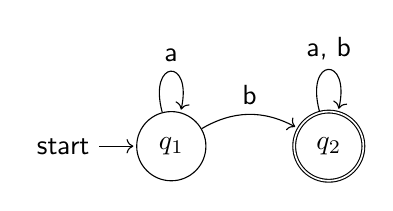
\begin{tikzpicture}[shorten >=1pt, node distance=2cm, on grid, auto]  
			\node[state, initial]    (q_0)   {$q_1$}; 
			\node[state, accepting] (q_1) [right=of q_0] {$q_2$};
			\path[->]
			(q_0) edge[loop above] node[align=center] {a} (q_0)
			(q_0) edge[bend left]  node[align=center] {b} (q_1)
			(q_1) edge[loop above] node[align=center]  {a, b} (q_1);
		\end{tikzpicture}
	}
\end{figure}

    \begin{enumerate}
        \item $Q=\{q_1, q_2\}$,
        \item $\Sigma = \{\texttt{a, b}\}$,
        \item $\delta$ = $\{\langle q_1, \texttt{a}, q_1 \rangle $, $\langle q_1, \texttt{b}, q_2 \rangle,$ $\langle q_2, \texttt{a}, q_2 \rangle,$ $\langle q_2, \texttt{b}, q_2 \rangle \}$,
        \item $q_1$ is the start state, and
        \item $F = \{q_2\}$
    \end{enumerate}
\end{frame}


\begin{frame}{Symbolic Automata}
% examples in application
    \begin{itemize}
        \setlength{\itemsep}{12pt}
         \item General \colorbf{Motivation}: Improve scaling for large alphabets
        \item Symbolic Automata (SFAs) are an extensions of FAs that replace explicit alphabets with predicates defined over a separate alphabet algebra
        \item \colorbf{Motivation} for \textcolor{umBlueLighter}{CER}:
        \vspace{0.6em}
            \begin{itemize}
            \setlength{\itemsep}{4pt}
                \item Unlike traditional FAs, SFAs can incorporate background knowledge through predicates
                \item SFAs allow for the use of a solver, which provides \textbf{logical facts}, includes \textbf{domain-specific axioms} and a \textbf{full-fledged inference engine} 
            \end{itemize}
    \end{itemize}
\end{frame}

\begin{frame}{Non-stationary Markov Chains}
    \begin{itemize}
        \setlength{\itemsep}{12pt}
         \item \textbf{Context}: We consider timeseries over a collection of random variables indexed by discrete-time 
         \item A \textcolor{umBlueLighter}{Markov chain} is a mathematical formulation that experiences \textbf{ probabilistic transitions} from one state to another
         \item \colorbf{Key Concept}: Only a limited number of previous observations are required to predict the future
         \item A Markov chain is \textbf{non-stationary} when the transitions are time-independent
    \end{itemize}
\end{frame}

\begin{frame}{Non-stationary Markov Chains and Automata}
    \begin{itemize}
        \setlength{\itemsep}{12pt}
         \item Markov chains can be modeled by FAs
         \item Adjustments:
         \vspace{0.6em}
            \begin{itemize}
            \setlength{\itemsep}{4pt}
                \item The start state is fixed and the chain \textbf{deterministically} starts from there
                % This probability is 0 when there is no transition from q to q' and is equal to or greater than 0 otherwise
                \item \textcolor{umBlueLighter}{Transition matrix $\Delta$} specifies the transition probabilities from one state to another
                \item $\delta$ vs $\Delta$ ?
                \item In a non-stationary Markov chain, $\Delta$ is \textbf{\textit{not constant}} over time
                \item We can compute the probability of the chain being in each state at any time point through recursive multiplication
            \end{itemize}
    \end{itemize}
\end{frame}

\begin{frame}{Neuro-symbolic\\ \hspace{0.6em} Artificial Intelligence}  % more like a goal
    \begin{tikzpicture}[remember picture,overlay]
    \node[inner sep=0pt, outer sep=90pt, anchor=left] at (current page.east) {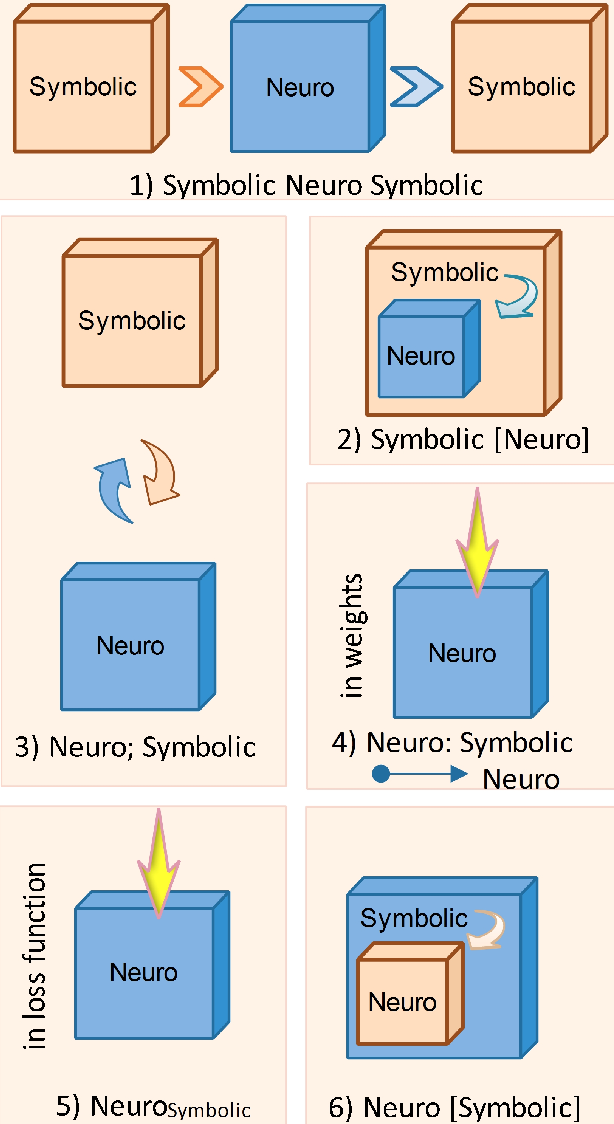
\includegraphics[width=0.25\paperwidth, height=\paperheight, keepaspectratio]{contents/images/NeSy.png}};
  \end{tikzpicture}
\end{frame}

\begin{frame}{Neuro-symbolic Artificial Intelligence}
    \begin{itemize}
        \setlength{\itemsep}{12pt}
        \item Neuro-symbolic Artificial Intelligence (NeSy) aims to merge \textbf{Knowledge Representation} (KR) and \textbf{Machine Learning} (ML)
        \item \colorbf{Motivation}: Leverage their respective strengths while mitigating their weaknesses
        \vspace{0.6em}
        \begin{itemize}
            \setlength{\itemsep}{4pt}
                \item KR has \textcolor{green!70!black}{strong theoretical foundations}, with analyses of expressivity, \textbf{\textit{tractability}}, their trade-offs, and the combination of multiple representations
                \item KR often struggles to deliver the desired  \textcolor{red!90!black}{performance} on practical tasks
                \item ML excels in \textcolor{green!70!black}{performance} but lacks \textcolor{red!90!black}{explainability} and reasoning behind its results [XAI]
            \end{itemize}
        \item \colorbf{Goals}: more \textbf{reliable}, \textbf{explainable} models with the ability to \textbf{generalize} to out-of-distribution data and require \textbf{fewer} training examples
        \item This integration is challenging $\rightarrow$ most of the SOTA methods are applied to toy tasks
    \end{itemize}
\end{frame}

\begin{frame}{Neuro-symbolic Artificial Intelligence}
    \begin{itemize}
        \setlength{\itemsep}{12pt}
        \item We are interested in a specific subset of NeSy:
        \vspace{1em}
        \begin{center}
            \textit{The \textbf{sequential integration} of a sub-symbolic module, specifically a neural network, with a symbolic module, specifically a symbolic automaton}
        \end{center}
        \item \colorbf{Why?} \textit{NN $\rightarrow$ simple events} \&  \textit{Automaton $\rightarrow$ complex events}
    \end{itemize}
\end{frame}


\begin{frame}{Probabilistic Inference and Weighted Model Counting}
%We borrow ideas from Statistical Relational Learning and Artificial Intelligence, which combines\\ \hspace{1em} logical and probabilistic reasoning
    \begin{itemize}
        \setlength{\itemsep}{11pt}
        \item In probabilistic reasoning, a scenario is modeled using a joint probability distribution over random variables, which is then used to answer probabilistic queries % finite domain random vars
        \item The joint distribution is sufficient to answer probabilistic queries, \textbf{\textit{but}} its size grows exponentially with the number of variables
        \item A procedure to perform probabilistic queries is \colorbf{Weighted Model Counting (WMC)}
        \item Given a probabilistic program, WMC \textbf{counts the solutions of a logical formula}, assigning each a \textbf{weight} based on importance or likelihood
        \item \textcolor{umBlueLighter}{How is it relevant to probabilistic inference?} It computes the probability of outcomes based on the weights of different models/interpretations
    \end{itemize}
\end{frame}

\begin{frame}{Tractable Boolean Circuits}
    \begin{itemize}
        \setlength{\itemsep}{12pt}
        \item WMC is generally intractable, thus exact some WMC use \textbf{knowledge compilation}
        \item Knowledge compilation maps the logical theory to a \textit{tractable representation}: a \colorbf{circuit}
        \item \textcolor{umBlueLighter}{Tractable Boolean Circuits} allow WMC queries to be answered in lin-time wrt. the size of the circuit 
        \item Their theory is based on \textbf{Negation Normal Form} (NNF) circuits, consisting of AND-gates, OR-gates, and inverters (which can only connect to circuit variables)
        \item  NNF circuits alone are not tractable, \textbf{\textit{but}} imposing certain properties enhance their tractability
        \item NNFs are \textbf{differentiable}, as they are composed of additions and multiplications
    \end{itemize}
\end{frame}

\begin{frame}{Tractable Boolean Circuits - Properties}
    \begin{itemize}
        \setlength{\itemsep}{12pt}
        \item \colorbf{Decomposability}: Circuit fragments feeding into an AND-gate cannot share variables [SAT]
        \item \colorbf{Determinism}: at most one input of an OR-gate can be evaluated to \texttt{True} for any given circuit input [MajSAT]
        \item \colorbf{Smoothness}: All circuit fragments feeding into an OR-gate to reference the same variables
        \item If NNF circuits are \textbf{decomposable}, \textbf{deterministic} and \textbf{smooth} they allow for solving the WMC problem in linear time
        \item \textit{Disclaimer}: We will use SDDs that are an extension of the previous
    \end{itemize}
\end{frame}

\iffalse
\begin{frame}{Tractable Boolean Circuits - Example} % forgive me for using electrical engineering terms
    \begin{columns}
        \begin{column}{0.4\textwidth}
            \begin{figure}[H]
                \centering
                \scalebox{0.73}{
                    \begin{circuitikz}[rotate=90,transform shape] \draw
                        % AND gate
                        (0,0) node[or port] (and1) {}
                        (0,-2) node[or port] (and2) {}
                        
                        % OR gate
                        (2,-1) node[and port] (or1) {}
                        
                        (-2,1.5) node[and port] (and3) {}
                        (-2,0) node[and port] (and4) {}
                        (-2,-1.5) node[and port] (and5) {}
                        (-2,-3) node[and port] (and6) {}
                        
                        (-4,1) node[or port] (or2) {}
                        (-4,-3.5) node[or port] (or3) {}
                        
                        (and3.in 1) node[below, rotate=270] (a) {$L$}
                        (or2.in 1) node[below, rotate=270] (b) {$K$}
                        (or2.in 2) node[below, rotate=270] (c) {$\neg K$}
                        (and4.in 1) node[below, rotate=270] (d) {$\neg L$}
                        (and4.in 2) node[below, rotate=270] (e) {$\bot$}
                        
                        (and5.in 1) node[below, rotate=270] (f) {$\neg P$}
                        (and5.in 2) node[below, rotate=270] (g) {$\neg A$}
                        (and6.in 1) node[below, rotate=270] (h) {$P$}
                        
                        (or3.in 1) node[below, rotate=270] (i) {$A$}
                        (or3.in 2) node[below, rotate=270] (j) {$\neg A$};
                        
                        \draw[black] (and1.out) -- ++(0.5,0) |- (or1.in 1);
                        \draw[black] (and2.out) -- ++(0.5,0) |- (or1.in 2);
                        
                        \draw[black] (and3.out) -- ++(0.5,0) |- (and1.in 1);
                        \draw[black] (and4.out) -- ++(0.5,0) |- (and1.in 2);
                        
                        \draw[black] (and5.out) -- ++(0.5,0) |- (and2.in 1);
                        \draw[black] (and6.out) -- ++(0.5,0) |- (and2.in 2);
                        
                        \draw[black] (or2.out) -- ++(0.5,0) |- (and3.in 2);
                        \draw[black] (or3.out) -- ++(0.5,0) |- (and6.in 2);
                    \end{circuitikz}
                }
            \end{figure}
        \end{column}

        % Right column with the itemized list
        \begin{column}{0.6\textwidth}
            \begin{itemize}
        \setlength{\itemsep}{18pt}
        \only<1->
        {\item \textbf{Decomposable?} {\small (Wires in AND-gates do not share variables)}}
        \only<2->
        {\hspace{0.5cm} \colorbf{Yes}}
        \only<3->
        {\item \textbf{Deterministic?} {\small (Max 1 wire in OR-gates \texttt{True} $\forall$ input)}}
        \only<4->
        {\hspace{0.5cm} \colorbf{Yes}}
        \only<5->
        {\item \textbf{Smooth?} {\small (All wires in OR-gates share variables) }}
        \only<6->
        {\hspace{0.5cm} \colorbf{No} $\dots$}
        \only<7->
        {\small \textit{How to enforce it?}}
    \end{itemize}
        \end{column}
    \end{columns}
\end{frame}
\fi

\begin{frame}{NeSy Inference and Training}
    \begin{itemize}
        \setlength{\itemsep}{12pt}
        \item Inference tasks can be transformed into the evaluation of a differentiable parametric circuit, which is in 1-to-1 correspondence with a probabilistic logic program
        \item The parameters are probabilities attached to the basic elements of a logical theory (facts or clauses)
        \item To perform NeSy inference we \textbf{reparameterize}: substitute the scalar values assigned to facts or formulas with the \textit{output of a neural network (NN)}
        \item Differentiable circuits with neural networks as leaves can be trained for probabilistic queries by maximizing the log-likelihood of training data via gradient descent
    \end{itemize}
\end{frame}


\section{Initial Dataset}
{
    \setbeamertemplate{headline}{}
    \begin{frame}
        \sectionpage%
        \begin{tikzpicture}[overlay,remember picture]
            \node[left=2cm] at (current page.2){%
                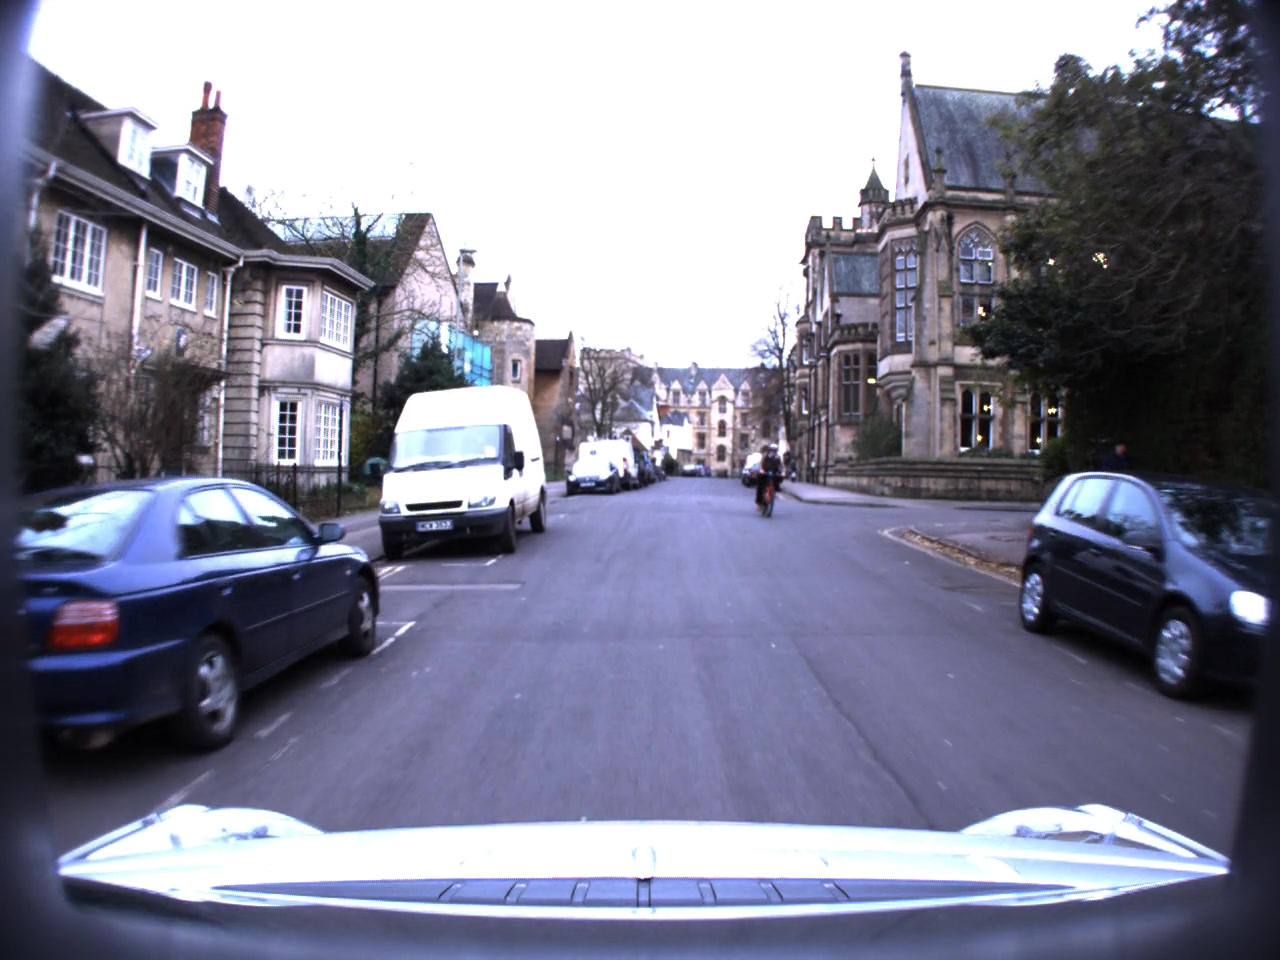
\includegraphics[width=5.5cm]{contents/images/05092.jpg}
            };
        \end{tikzpicture}
    \end{frame}
}

\begin{frame}{ROAD-R Dataset}
    \begin{itemize}
        \setlength{\itemsep}{12pt}
        \item There is a plethora of autonomous driving vision datasets
        \item ROAD is a real-world dataset with \textcolor{umBlueLighter}{22}, \textcolor{umBlueLighter}{8-minute} long videos from the view of an \textbf{autonomous vehicle (AV)}
        \item The videos were recorded over the period of November 2014 to December 2015, by traversing through central Oxford 
        \item  ROAD-R is enhanced with \textcolor{umBlueLighter}{243} requirements in propositional logic to capture \textbf{background knowledge} 
        \vspace{4pt}
        \begin{itemize}
            \item \textit{e.g. $\neg (red\_light \wedge green\_light)$ }$\equiv$ a traffic light cannot simultaneously display \textcolor{red}{red} \&  \textcolor{green!60!black}{green} 
        \end{itemize}
        \item The total number of annotated frames is $\sim$ 122K ($\sim$ 12 frame/sec)
    \end{itemize}
\end{frame}


\begin{frame}{ROAD-R Dataset}
    \begin{itemize}
        \setlength{\itemsep}{13pt}
        \item Each video is annotated with a \textcolor{umBlueLighter}{series of bounding boxes} (per frame) \textbf{linked in time} including:
        \vspace{4pt}
        \begin{itemize}
            \setlength{\itemsep}{4pt}
            \item the label associated with the \textbf{agent} \textit{e.g. “Pedestrian”}
            \item the \textbf{action(s)} the agent is doing \textit{e.g., “Moving Away”} 
            \item the \textbf{semantic location(s)} where the agent is placed \textit{e.g., “Incoming Lane”}
        \end{itemize}
        \item Regarding AV itself, we only know its \textbf{ego-action}
    \end{itemize}
\end{frame}


\begin{frame}{Agents}
  \begin{multicols}{2}
        \begin{enumerate}
            \setlength\itemsep{1em}
            \item Pedestrian
            \item Car
            \item Cyclist
            \item Motorbike
            \item Medium vehicle
            \item Large vehicle
            \item Bus
            \item Emergency vehicle
            \item AV traffic light 
            \item Other traffic light
        \end{enumerate}
    \end{multicols}
\end{frame}


\begin{frame}{Actions}
Actions available for the \colorbf{AV}:
  \begin{multicols}{4}
        \begin{enumerate}
            \setlength\itemsep{0.4em}
            \item Stop
            \item Move
            \item Turn right
            \item Turn left
            \item Move right
            \item Move left
            \item Overtake
        \end{enumerate}
    \end{multicols}
Actions available for the \colorbf{agents}:
  \begin{multicols}{4}
        \begin{enumerate}
            \setlength\itemsep{0.4em}
            \item Move away
            \item Move towards
            \item Move
            \item Brake
            \item Stop
            \item Indicating left
            \item Indicating right
            \item Hazards lights on
            \item Turn left
            \item Turn right
            \item Overtake
            \item Push object
            \item Wait to cross
            \item Cross from left
            \item Cross from right
            \item Crossing
            \item Red traffic light
            \item Green traffic light
            \item Amber traffic light
        \end{enumerate}
    \end{multicols}
\end{frame}

\begin{frame}{Locations}
  \begin{multicols}{2}
        \begin{enumerate}
            \setlength\itemsep{1em}
            \item AV lane
            \item Outgoing lane
            \item Outgoing cycle lane
            \item Incoming lane
            \item Incoming cycle lane
            \item Pavement
            \item Left pavement
            \item Right pavement
            \item Junction
            \item Crossing location
            \item Bus stop
            \item Parking
        \end{enumerate}
    \end{multicols}
\end{frame}

% This one for complexity
{
 \setbeamertemplate{headline}{}
\begin{frame}{Annotated\\ \hspace{0.7em} Example 1}
    \begin{tikzpicture}[remember picture,overlay]
    \node[inner sep=0pt, outer sep=0pt, anchor=left] at (current page.east) {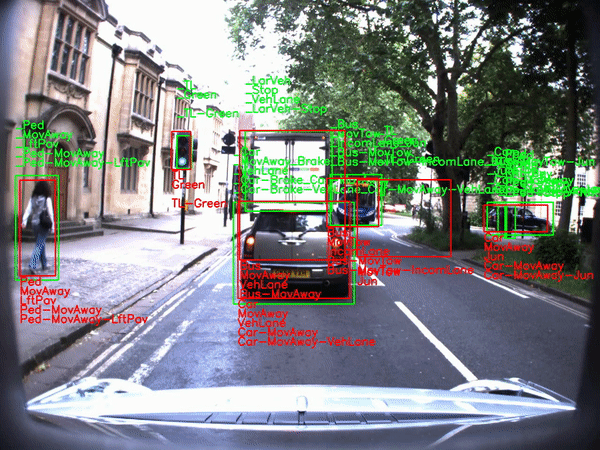
\includegraphics[width=0.67\paperwidth, height=\paperheight, keepaspectratio]{contents/images/short_clip.png}};
  \end{tikzpicture}
\end{frame}
}

% This one for explanation
{
 \setbeamertemplate{headline}{}
\begin{frame}{Annotated\\ \hspace{0.7em} Example 2}
    \begin{tikzpicture}[remember picture,overlay]
    \node[inner sep=0pt, outer sep=0pt, anchor=left] at (current page.east) {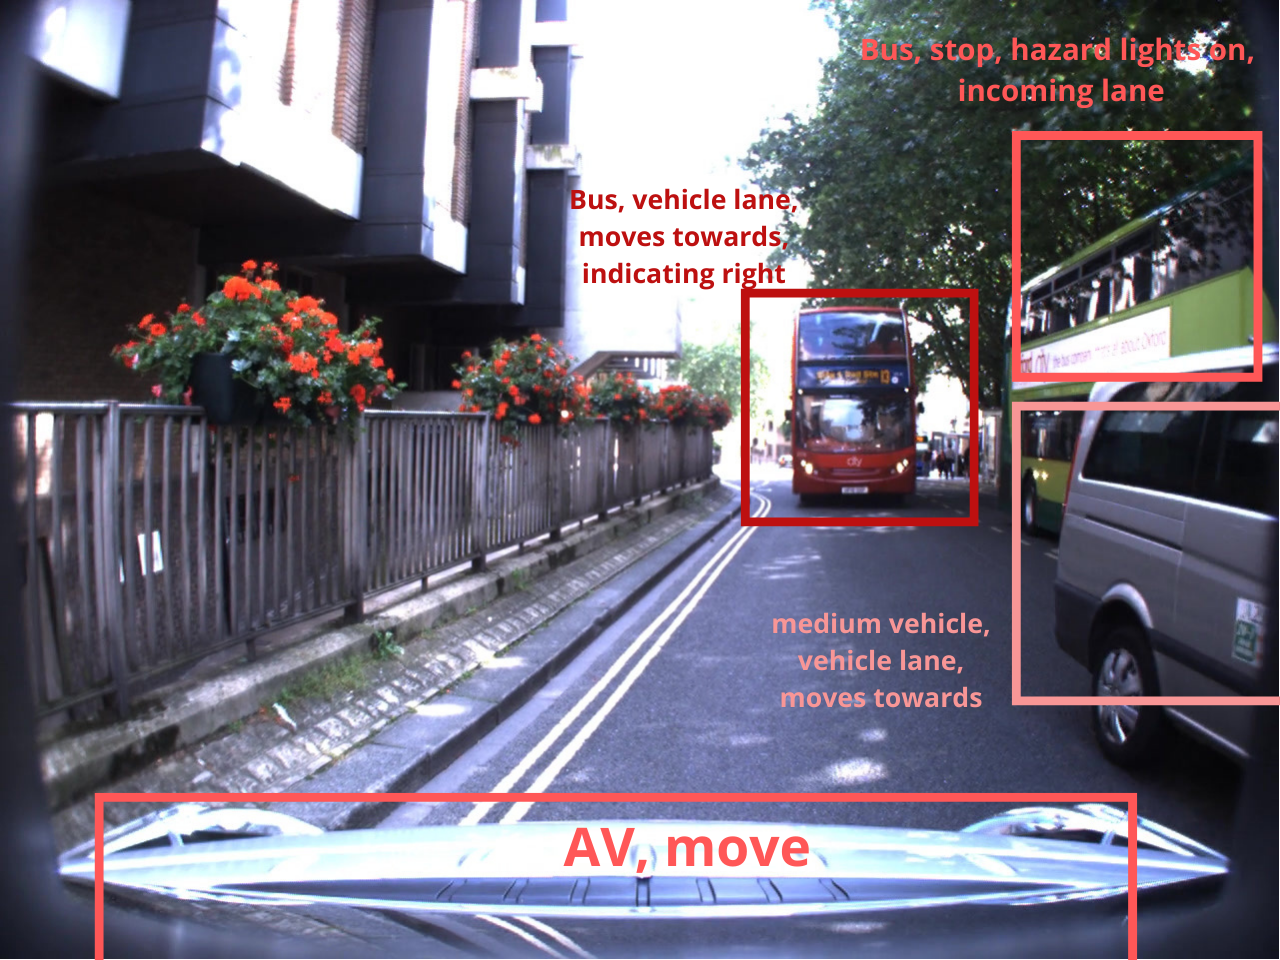
\includegraphics[width=0.67\paperwidth, height=\paperheight, keepaspectratio]{contents/images/annot_frame.png}};
  \end{tikzpicture}
\end{frame}
}


%%%%%%%%%%%%%%%%%%%%%%%%%%%%%%%%%%%%
%% SECTION PAGE: without background image
%%
%\section{Overtake}
%{
%    \setbeamertemplate{headline}{}
%    \begin{frame}
%        \sectionpage%
%        \begin{tikzpicture}[overlay,remember picture]
%            \node[left=2cm] at (current page.2){%
%                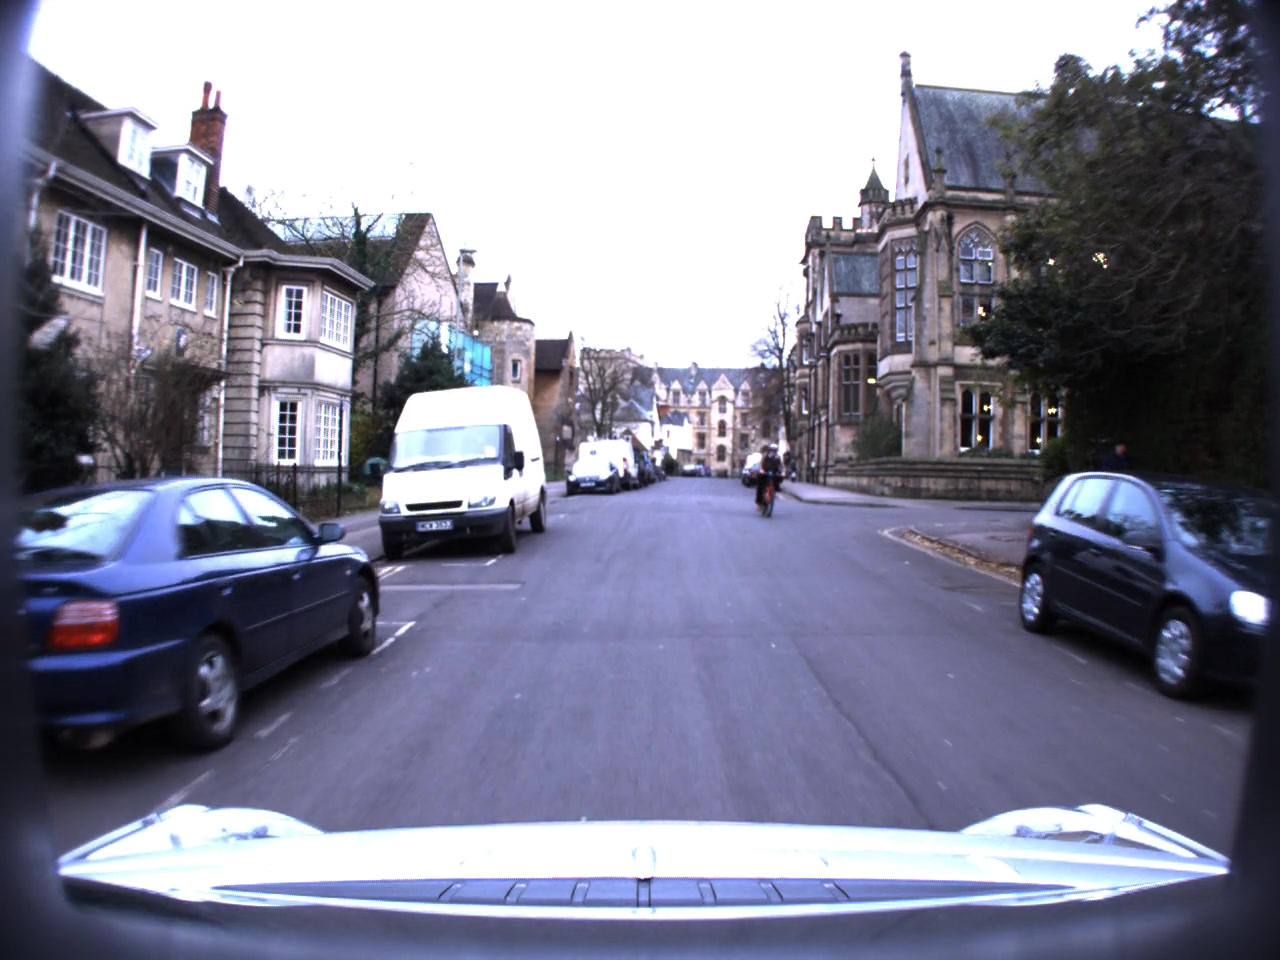
\includegraphics[width=5.5cm]{contents/images/05092.jpg}
%            };
%        \end{tikzpicture}
%    \end{frame}
%}

\begin{frame}{Overtake Action}
    \begin{itemize}
        \setlength{\itemsep}{13pt}
        \item Annotated actions differ from each other in terms of complexity
        \vspace{4pt}
        \begin{itemize}
            \item \textit{e.g.} actions regarding the traffic lights are more like states
        \end{itemize}
        \item The \textbf{overtake} action can be seen as a \textbf{complex event} in terms of CER, in a sense that:
        \vspace{0.6em}
            \begin{itemize}
            \setlength{\itemsep}{4pt}
                \item it may consist of simpler events
                \item its end is significantly different than the start
            \end{itemize}
        \item It, also, is an important complex event in the autonomous driving domain
        \item \textit{The predictive task of this thesis is the recognition of this complex event}
    \end{itemize}
\end{frame}

\begin{frame}{Some `Overtake' Information}
    \begin{itemize}
        \setlength{\itemsep}{10pt}
        \item  The unique overtake events in the dataset are \textcolor{umBlueLighter}{28 (+2)} in total :
        \vspace{4pt}
        \begin{itemize}
            \setlength{\itemsep}{3pt}
            \item \textcolor{umBlueLighter}{10}, where the \textbf{AV performs} the overtake
            \item \textcolor{umBlueLighter}{18}, where \textbf{other agents perform} the overtake
        \end{itemize}
        \item The duration of an overtake event, i.e. \textbf{number of frames}, varies from \textcolor{umBlueLighter}{2 to 164}
        \vspace{4pt}
        \begin{itemize}
            \item mean \#frames is \textit{49.83} and std is \textit{41.87}
        \end{itemize}
        \item We only know from the annotation who performs the overtake, \textbf{not} who is `overtaken'
        \item We watched all the overtake events and observed that the agents that :
        \vspace{4pt}
        \begin{itemize}
            \setlength{\itemsep}{3pt}
            \item \textbf{Perform the overtake} are mostly the \textcolor{umBlueLighter}{AV}, \textcolor{umBlueLighter}{cyclists}, \textcolor{umBlueLighter}{cars} and \textcolor{umBlueLighter}{medium vehicles}
            \item Are \textbf{overtaken} are primarily the \textcolor{umBlueLighter}{buses}, \textcolor{umBlueLighter}{large vehicles} and \textcolor{umBlueLighter}{cars} 
        \end{itemize}
    \end{itemize}
\end{frame}

\begin{frame}{`Overtake' examples}
    \begin{itemize}
        \setlength{\itemsep}{14pt}
        \item  Overtake incidents \textbf{vary significantly}, i.e., the patterns that form a complex event are diverse
        \item \textcolor{umBlueLighter}{Examples :}
    \end{itemize}
\end{frame}


\begin{frame}{}
       \begin{figure}
        \centering
        \begin{subfigure}{0.46\textwidth}
            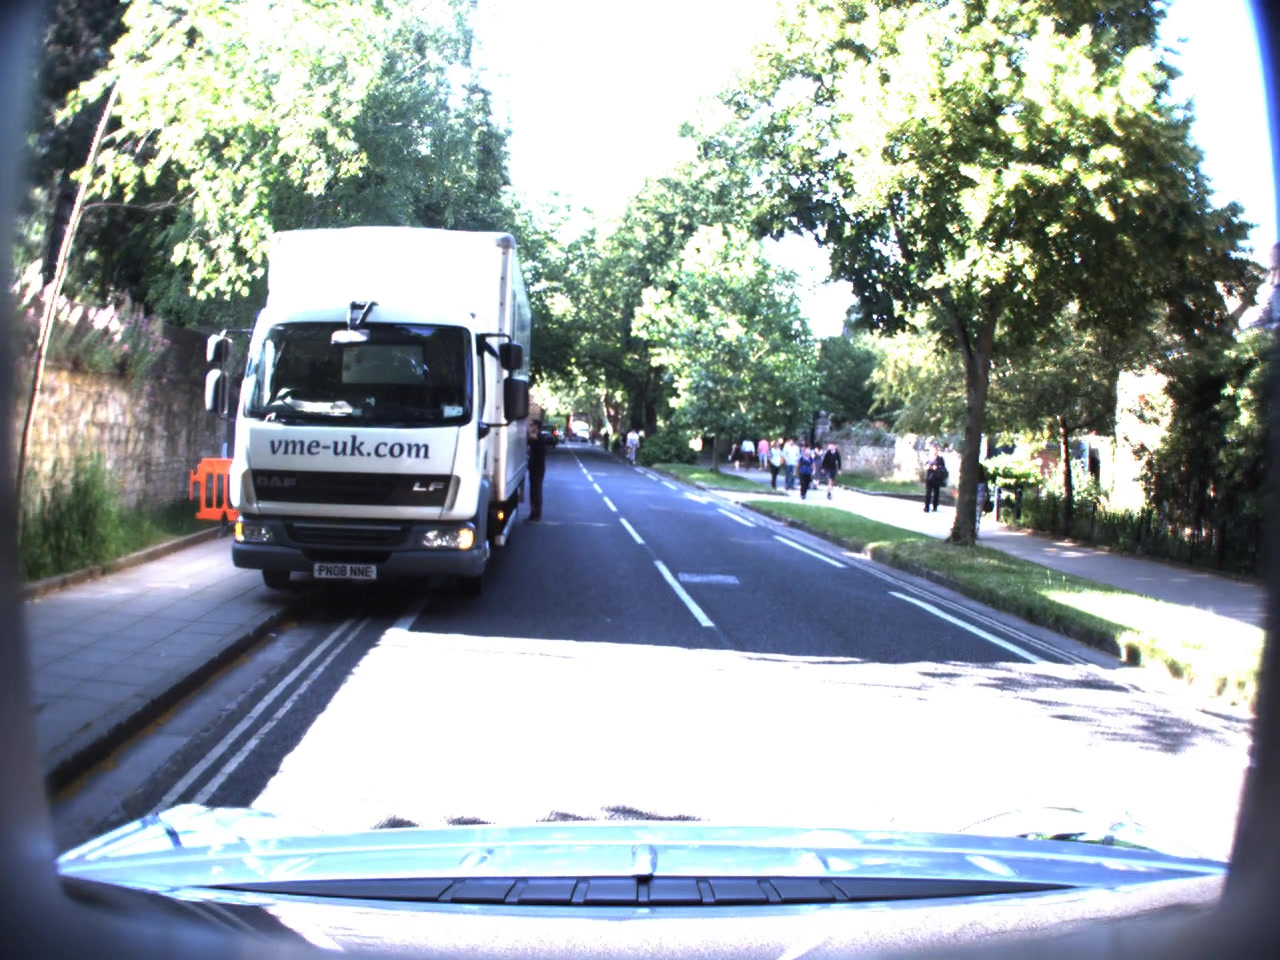
\includegraphics[width=\textwidth]{contents/images/ex1/00153.jpg}
        \end{subfigure}
        \hfill
        \begin{tikzpicture}[overlay]
        \draw[->, line width=1mm, UmBlueDarker] (-0.48,2.3) -- (0.48,2.3); 
        \end{tikzpicture}
        \hfill
        \begin{subfigure}{0.46\textwidth}
            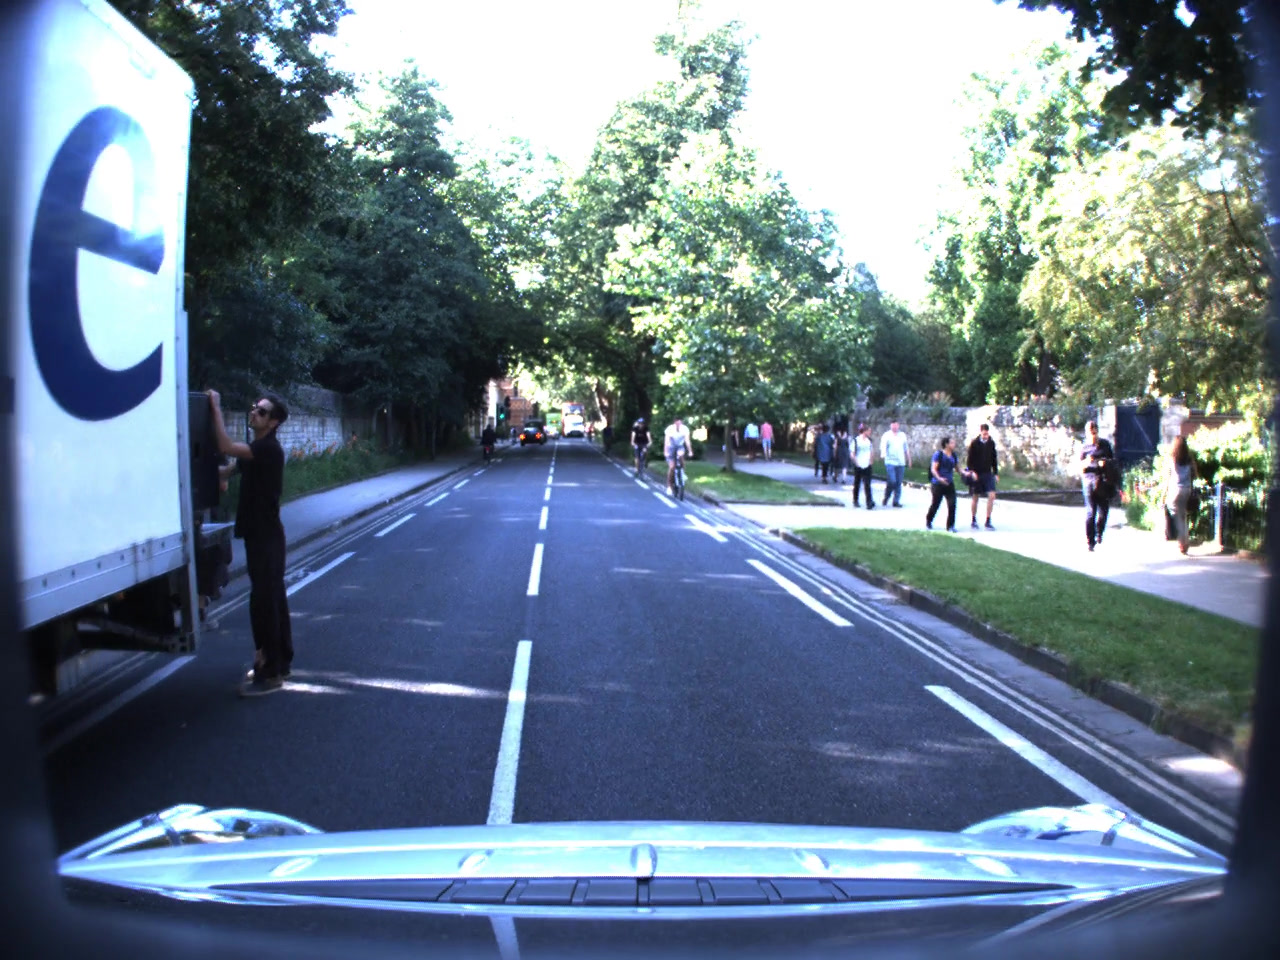
\includegraphics[width=\textwidth]{contents/images/ex1/00192.jpg}
        \end{subfigure}
    \end{figure}
\end{frame}

\begin{frame}{}
       \begin{figure}
        \centering
        \begin{subfigure}{0.46\textwidth}
            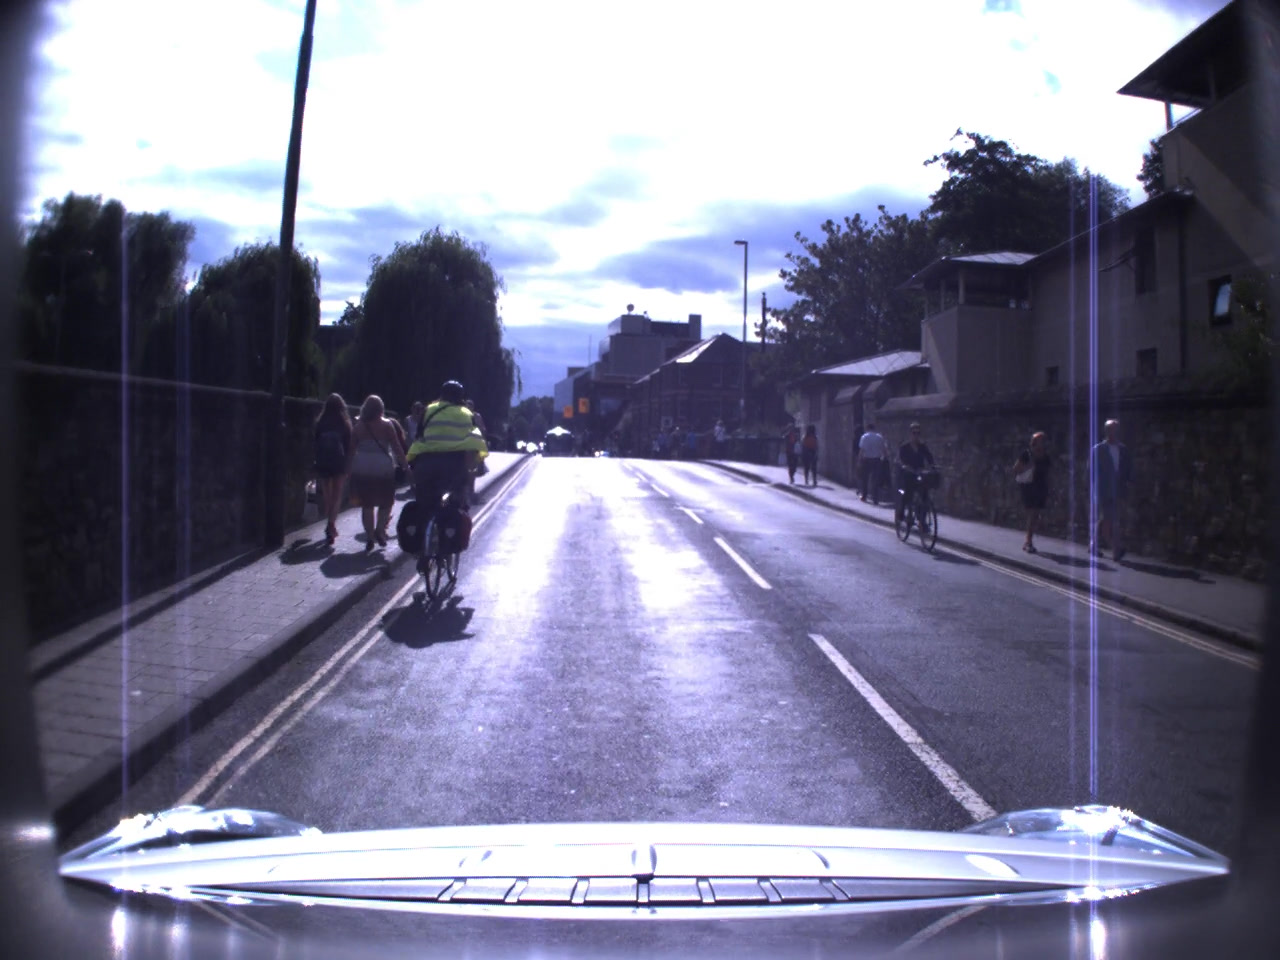
\includegraphics[width=\textwidth]{contents/images/ex2/01093.jpg}
        \end{subfigure}
        \hfill
        \begin{tikzpicture}[overlay]
        \draw[->, line width=1mm, UmBlueDarker] (-0.48,2.3) -- (0.48,2.3); 
        \end{tikzpicture}
        \hfill
        \begin{subfigure}{0.46\textwidth}
            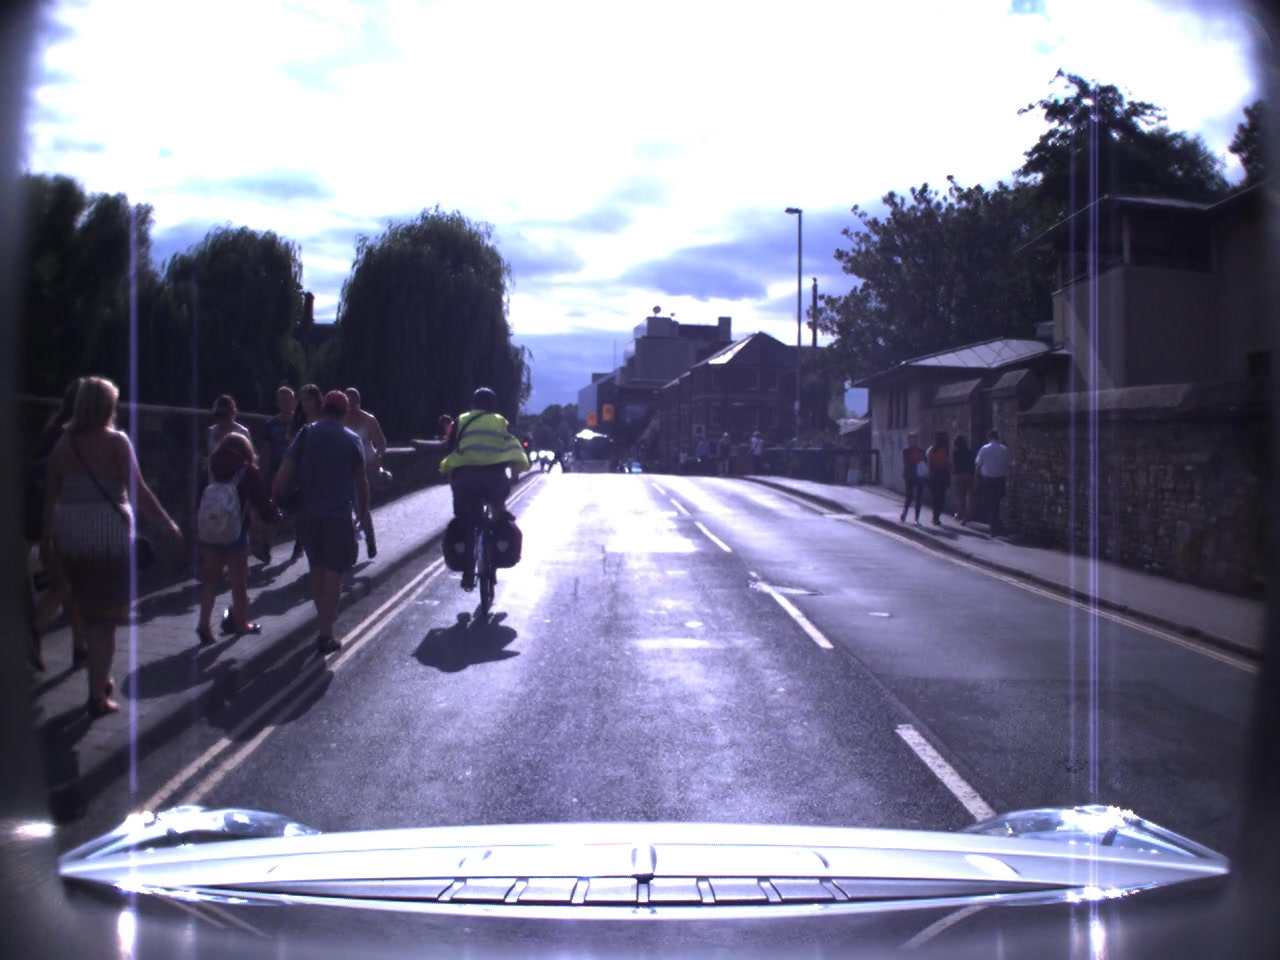
\includegraphics[width=\textwidth]{contents/images/ex2/01115.jpg}
        \end{subfigure}
    \end{figure}
\end{frame}


\begin{frame}{}
       \begin{figure}
        \centering
        \begin{subfigure}{0.46\textwidth}
            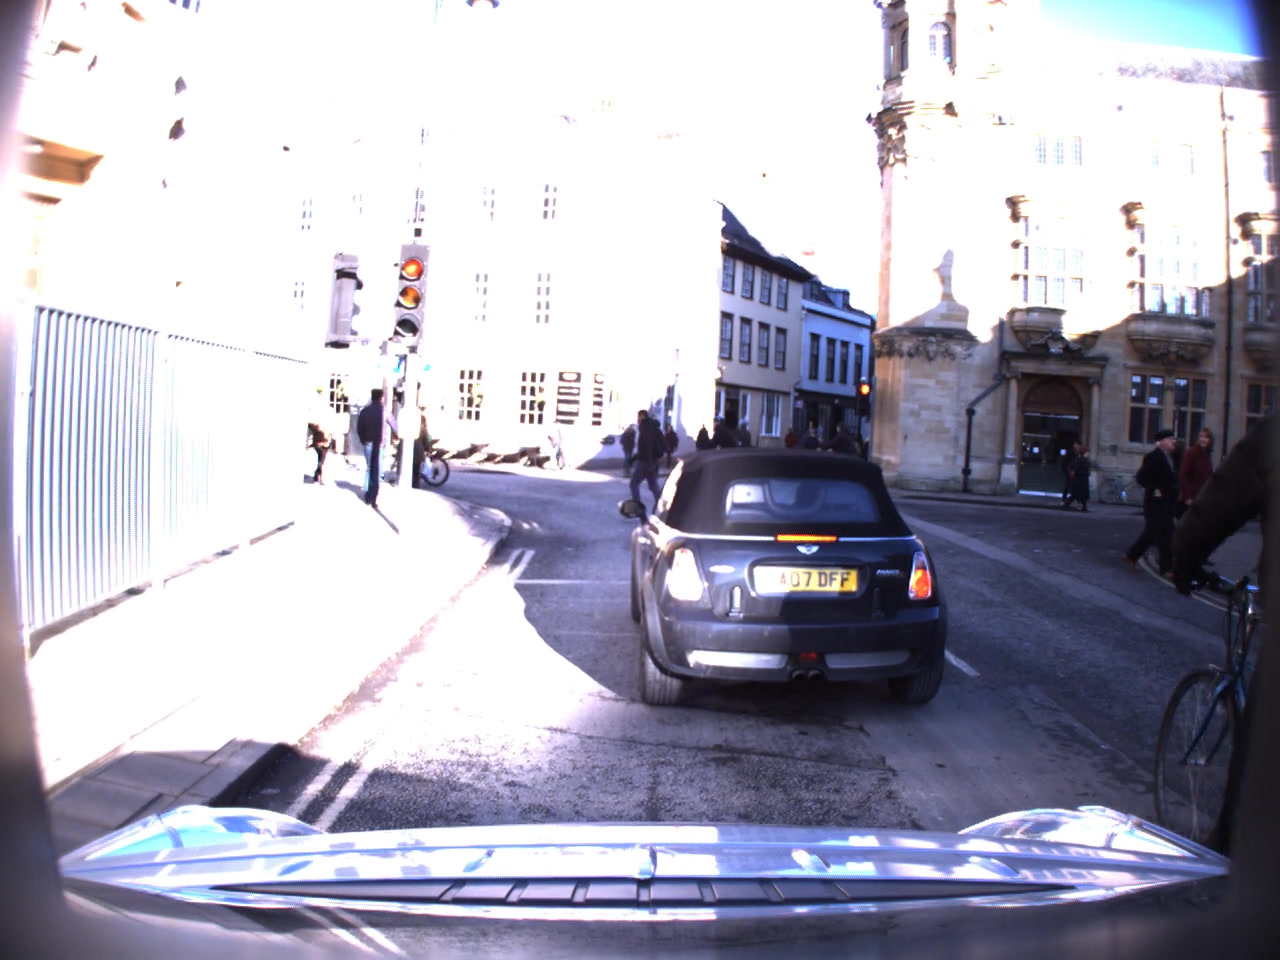
\includegraphics[width=\textwidth]{contents/images/ex3/02744.jpg}
        \end{subfigure}
        \hfill
        \begin{tikzpicture}[overlay]
        \draw[->, line width=1mm, UmBlueDarker] (-0.48,2.3) -- (0.48,2.3); 
        \end{tikzpicture}
        \hfill
        \begin{subfigure}{0.46\textwidth}
            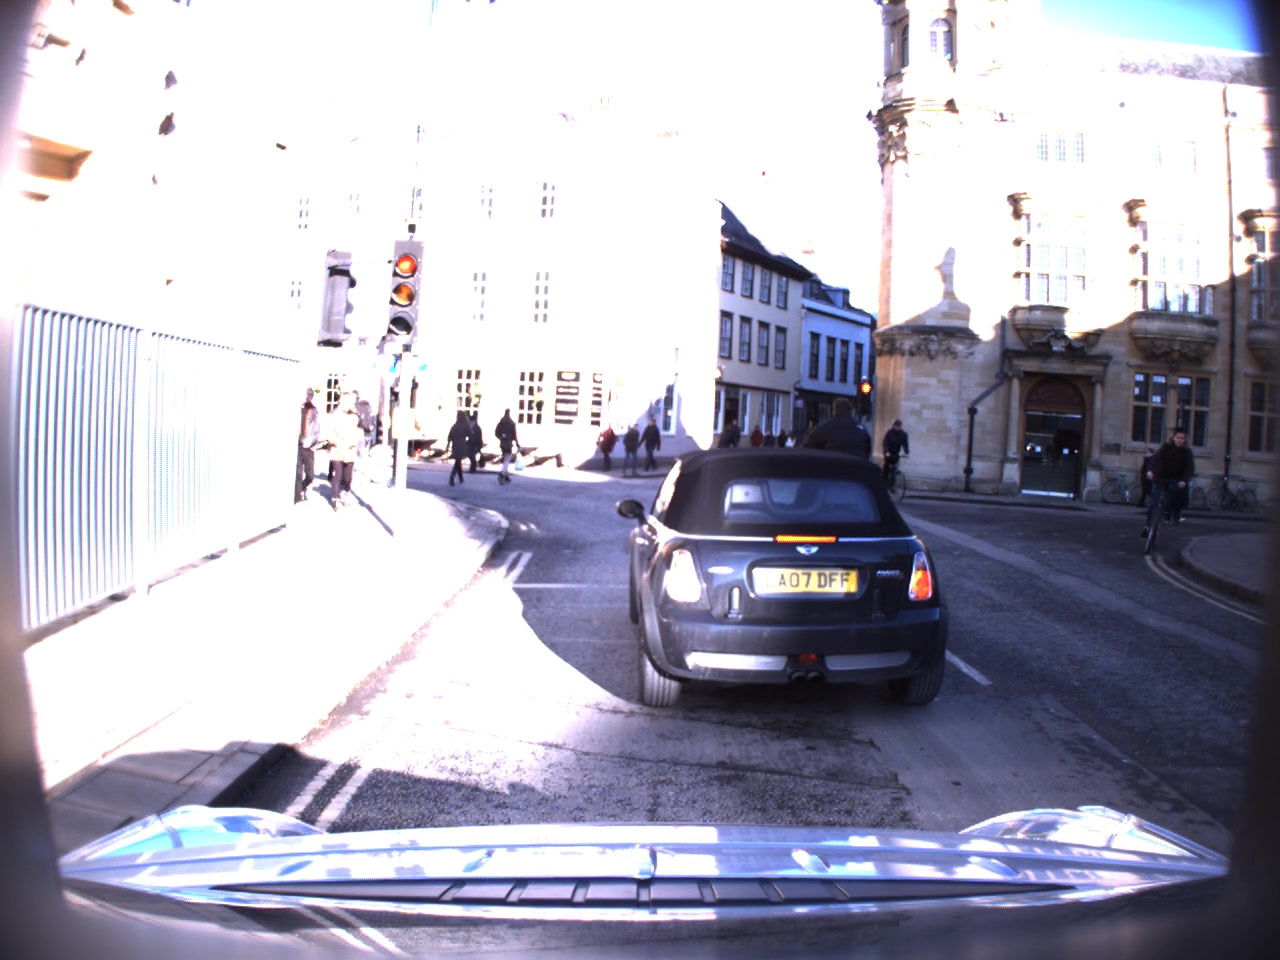
\includegraphics[width=\textwidth]{contents/images/ex3/02784.jpg}
        \end{subfigure}
    \end{figure}
\end{frame}

\begin{frame}{Re-cap and Motivation Moving Forward}
       \begin{enumerate}
        \setlength{\itemsep}{10pt}
        \item CER on video data
        \item NN for actions and locations, symbolic automaton for `overtake' recognition
        \item `Overtake' patterns are not available $\rightarrow$ we need to \textbf{learn them}
        \item From ROAD-R, we derive a \textbf{symbolic dataset} to learn `overtake' automata
        \item We translate the automata to probabilistic automata through Markov chains
        \item The probabilistic program is compiled to a differentiable circuit 
        \item Through the circuit probabilistic queries are answered
        \item Loss is computed and propagated
    \end{enumerate}
\end{frame}


\section{Sequential Datasets}
{
    \setbeamertemplate{headline}{}
    \begin{frame}
        \sectionpage%
        \begin{tikzpicture}[overlay,remember picture]
            \node[left=2cm] at (current page.2){%
                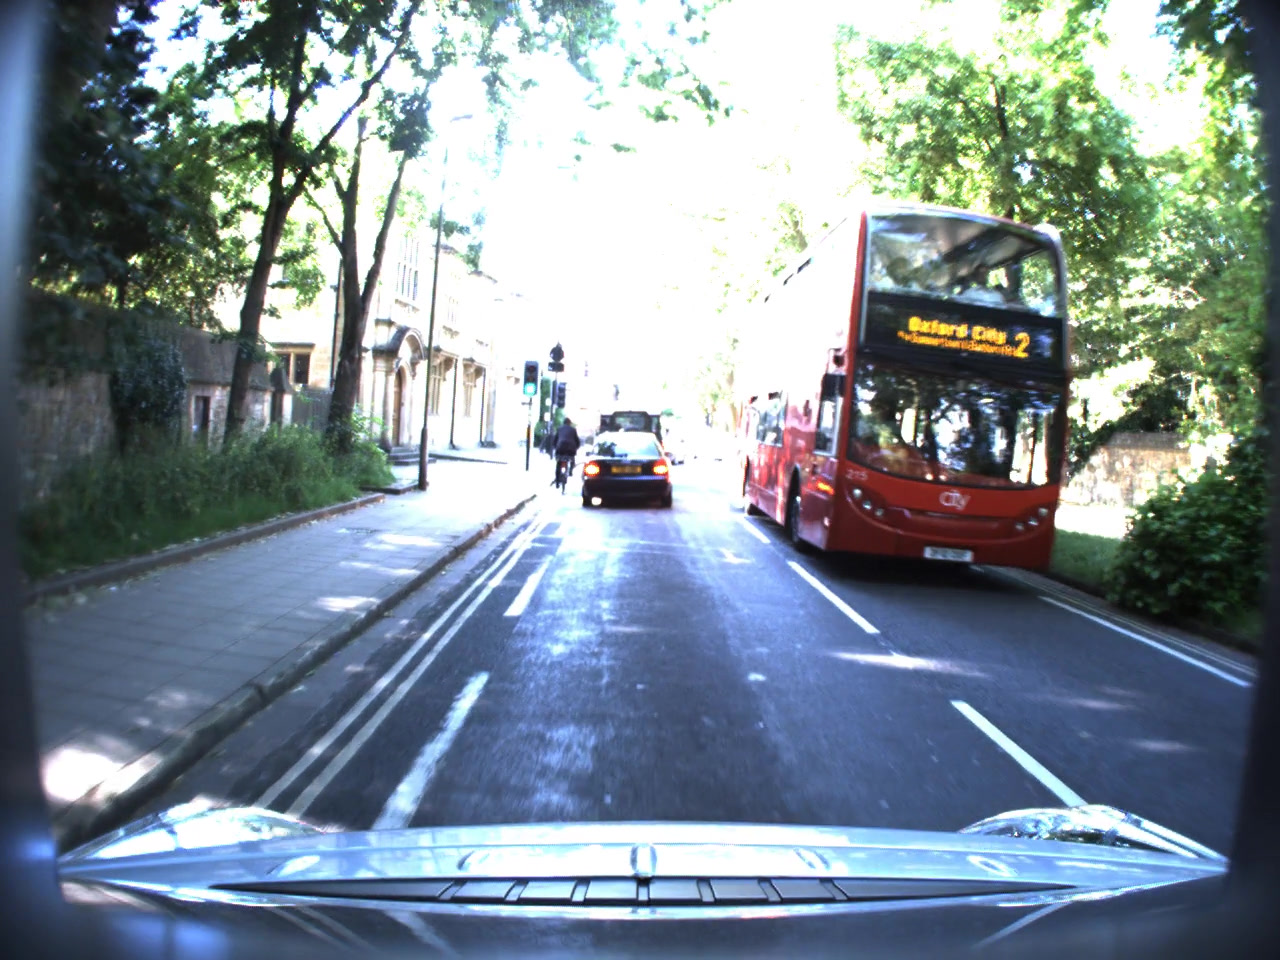
\includegraphics[width=5.5cm]{contents/images/00363}
            };
        \end{tikzpicture}
    \end{frame}
}

\begin{frame}{Sequential Datasets}
    \begin{itemize}
        \setlength{\itemsep}{12pt}
        % To lew kataxristika ROAD-R
        \item  From ROAD, we created a \colorbf{symbolic} sequential dataset and a \colorbf{sub-symbolic} one 
        \item  They model whether the example involves the AV (\textit{we use the subset that does not consider the AV}) % as it is adifferent vision problem
        \item The datasets consist of sequences  and provide \textcolor{umBlueLighter}{2 agents'}:
        \vspace{6pt}
        \begin{itemize}
            \setlength{\itemsep}{3pt}
            \item \textbf{Identity} \textit{e.g. av, larveh}
            \item \textbf{Action} per timepoint/frame
            \item \textbf{Semantic location} per timepoint/frame
            \item \textbf{Coordinates} (normalized bounding box) per timepoint/frame
        \end{itemize}
        \vspace{6pt}
        and the example's \textbf{class} (which considers who has overtaken who)
        \item One dataset has the info encoded into \textbf{logical facts} and the other includes \textbf{images}
    \end{itemize}
\end{frame}



\begin{frame}{Positive Instances}
% Range is from 6 to 10 for a reason
    \begin{itemize}
        \setlength{\itemsep}{13pt}
        \item To generate the positive instances, we first chose a  maximum sequence length of 10
        \item Then, from the overtake instance we got chunks of frames of \textbf{minimum length 6} and\textbf{ maximum 10} with 5 frames in between the chunks (less for smaller instances)
        \item This process resulted in \textcolor{umBlueLighter}{92 positive instances}  which all end with an overtake action
    \end{itemize}
\end{frame}


\begin{frame}{Negative Instances}
    \begin{itemize}
        \setlength{\itemsep}{10pt}
        \item  In theory, all pairs of agents not involved in an overtake can be a negative example
        \item However, we investigated \textbf{close negatives}; negatives that look like they are going to lead to an overtake, but will not
        \item So, we collected \textbf{all action pairs that precede} an overtake and sampled agent-pair sequences that perform these actions, but \textbf{are not involved in an overtake}
        \item This resulted in \textcolor{umBlueLighter}{$\sim$ 5,500 negative} instances
    \end{itemize}
\end{frame}


\begin{frame}{Balancing the Dataset}
    \begin{itemize}
        \setlength{\itemsep}{10pt}
        \item  At this point, the dataset is highly \textbf{imbalanced} as the positive examples are only the \textit{\%1.6} of the total dataset
        \item Therefore, to balance the dataset we :
        \vspace{5pt}
        \begin{itemize}
            \setlength{\itemsep}{3pt}
            \item Made sure each agent-pair is \textbf{unique} $\rightarrow$ \textcolor{umBlueLighter}{$\sim$ 2,500}
            \item Considered sequences where both agents appear \& with \textbf{min length of 6} $\rightarrow$ \textcolor{umBlueLighter}{$\sim$ 2,000}
        \end{itemize}
        \item Can we balance it more? \colorbf{No.} \textit{Why?}
        \vspace{5pt}
        \begin{itemize}
            \setlength{\itemsep}{3pt}
            \item Not representative of the real world
            \item \textbf{Still a computer vision problem!}
        \end{itemize}
    \end{itemize}
\end{frame}

\begin{frame}{Train and Test splits}
    \begin{itemize}
        \setlength{\itemsep}{10pt}
        \item We will use the whole symbolic dataset to learn the `overtake' automata
        \item For the NeSy training, we need to split the sub-symbolic dataset into \textbf{train/test} sets
        \item We need to assure these sets \textit{do not intersect} : 
        \vspace{5pt}
        \begin{itemize}
            \setlength{\itemsep}{3pt}
            \item No positive instances from the same augmentation of positive examples in both sets 
            \item No negative instances from the same part of the video in both sets 
        \end{itemize}
        \item So, we reserved positives from some videos for training and used the rest for testing \textcolor{umBlueLighter}{\small (\textit{Why not for negatives? Again, computer vision!})}
        \item We do a \%80/\%20 split with k-folds, resulting in 36 set pairs where 24 are useful 
        \vspace{5pt}
        \begin{itemize}
            \setlength{\itemsep}{3pt}
            \item \#positive sequences $\rightarrow$ training:  \textbf{46 -- 75}, testing: \textbf{17 -- 46} % Still pretty imbalanced
            \item \#negative sequences$\rightarrow$ training: $\sim$ 550, testing: $\sim$ 250 
        \end{itemize}
    \end{itemize}
\end{frame}


\section{Automata Learning}
{
    \setbeamertemplate{headline}{}
    \begin{frame}
        \sectionpage%
        \begin{tikzpicture}[overlay,remember picture]
            \node[left=2cm] at (current page.2){%
                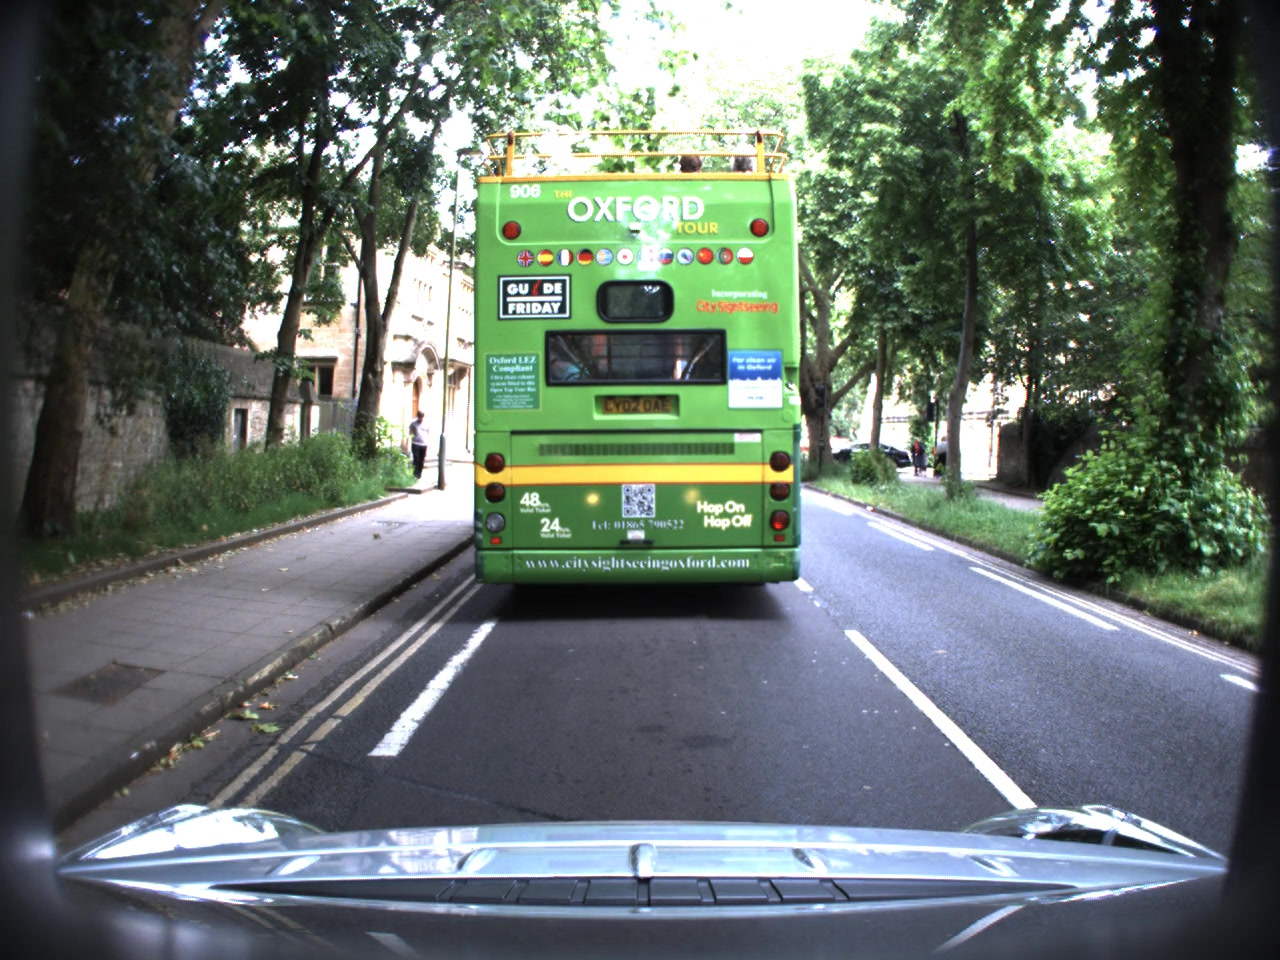
\includegraphics[width=5.5cm]{contents/images/00052}
            };
        \end{tikzpicture}
    \end{frame}
}


\begin{frame}{Learn `overtake' Patterns}
    \begin{itemize}
        \setlength{\itemsep}{13pt}
        \item Automata model patterns that define complex events in CER
        \item For `overtake' incidents, patterns are learned from the symbolic dataset, simulating \textbf{expert knowledge}
        \item We use \textit{ASAL framework} to learn symbolic automata from data, without needing perfect discrimination between positive and negative examples
        \item The \textcolor{umBlueLighter}{entire dataset} was used for learning, instead of training/testing splits, to mimic expert-provided background knowledge (\textit{our primary goal is NeSy integration})
        % our primary goal is neurosymbolic integration, not the evaluation of automata induction performance, thus no evaluation set is required
    \end{itemize}
\end{frame}

\begin{frame}{`Overtake' Automata}
    \begin{itemize}
    \setlength{\itemsep}{10pt}
    \item Transitions in the learned automata use only combinations of \textbf{actions} and \textbf{locations}
    \item Agent identity is excluded to avoid overfitting
    \item Initially, the algorithm had freedom to learn patterns from the simple event sets and discovered meaningful patterns using a \textit{subset} of simple events:
    \vspace{5pt}
    \begin{itemize}
        \setlength{\itemsep}{3pt}
        \item \textbf{Actions}: Moving away (\texttt{movaway}), Stop, other
        \item \textbf{Locations}: Incoming lane (\texttt{incomlane}), Vehicle lane (\texttt{vehlane}), Junction (\texttt{jun}), other
    \end{itemize}
    \item These subsets were then fixed, restricting the algorithm to them for further learning
    \item We learned \colorbf{3 automata}, equally good at discrimination but with different purposes
    \item Their F1-score is $\sim$ \textit{0.97}, with TPs (92), FPs (5) \& no FNs
\end{itemize}
\end{frame}

\begin{frame}{Automaton 1 - Simple}
    \begin{columns}
        \column{0.5\textwidth}
        \centering
        \scalebox{0.63}{
            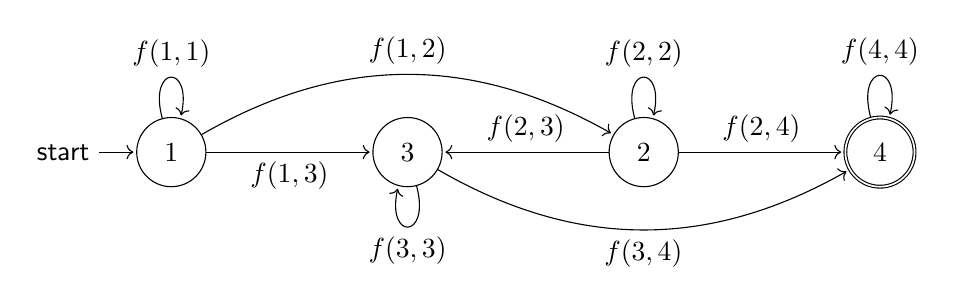
\begin{tikzpicture}[shorten >=1pt, node distance=3cm, on grid, auto]  
                \node[state, initial] (q_0)   {$1$}; 
                \node[state] (q_2) [right=of q_0] {$3$};
                \node[state] (q_1) [right=of q_2] {$2$}; 
                \node[state, accepting] (q_3) [right=of q_1] {$4$}; 
                \path[->]
                (q_0) edge[loop above] node[align=center] {$f(1,1)$} (q_0)
                (q_0) edge                  node[align=center, below] {$f(1,3)$} (q_2)
                (q_0) edge[bend left, looseness=1] node[align=center] {$f(1,2)$} (q_1)
                
                (q_1) edge[loop above]      node[align=center]  {$f(2,2)$} (q_1)
                edge                  node[align=center, above] {$f(2,3)$} (q_2)
                edge                  node[align=center, above] {$f(2,4)$} (q_3)
                (q_2) edge[loop below]      node {$f(3,3)$} (q_2)
                edge[bend right, looseness=1]       node[below] {$f(3,4)$} (q_3)
                (q_3) edge[loop above]      node {$f(4,4)$} (q_3); 
            \end{tikzpicture}
        }

        \column{0.5\textwidth}
         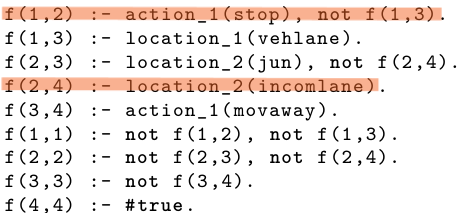
\includegraphics[width=\textwidth]{contents/images/autom_1.png}
    \end{columns}
\end{frame}

\begin{frame}{Automaton 2 - Complex}
    \begin{columns}
        \column{0.48\textwidth}
        \centering
        \scalebox{0.65}{
            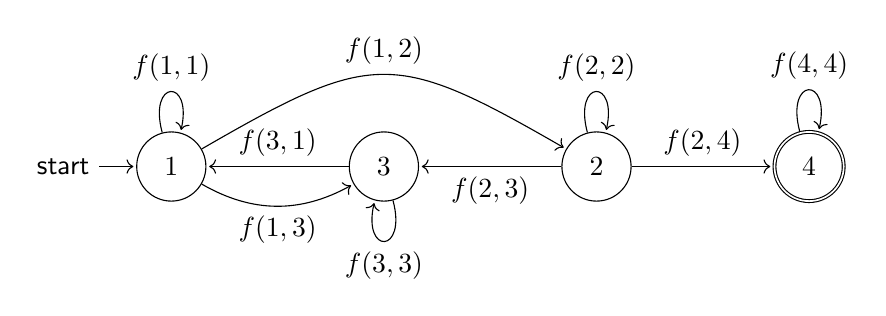
\begin{tikzpicture}[shorten >=1pt, node distance=2.7cm, on grid, auto]  
				\node[state, initial] (q_0)   {$1$}; 
				\node[state] (q_2) [right=of q_0] {$3$};
				\node[state] (q_1) [right=of q_2] {$2$}; 
				\node[state, accepting] (q_3) [right=of q_1] {$4$}; 
				\path[->]
				(q_0) edge[loop above] node[align=center] {$f(1,1)$} (q_0)
				(q_0) edge[bend right] node[align=center, below] {$f(1,3)$} (q_2)
				(q_0) edge[bend left, looseness=1.4] node[align=center] {$f(1,2)$} (q_1)
				(q_1) edge[loop above] node[align=center] {$f(2,2)$} (q_1)
				edge node[align=center, below] {$f(2,3)$} (q_2)
				edge node[align=center, above] {$f(2,4)$} (q_3)
				(q_2) edge[loop below] node {$f(3,3)$} (q_2)
				edge node[above] {$f(3,1)$} (q_0)
				(q_3) edge[loop above] node {$f(4,4)$} (q_3); 
			\end{tikzpicture}
        }
        \column{0.52\textwidth}
         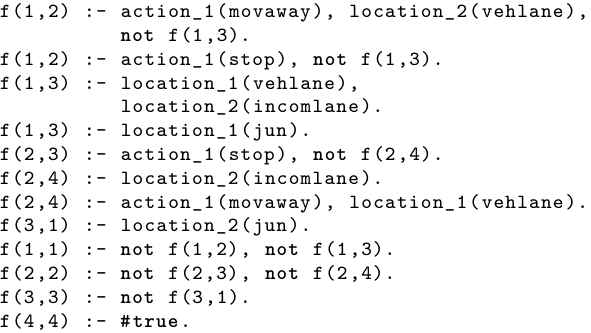
\includegraphics[width=\textwidth]{contents/images/autom_2.png}
    \end{columns}
\end{frame}

\begin{frame}{Automaton 3 - Complex with `other'}
    \begin{columns}
        \column{0.48\textwidth}
        \centering
        \scalebox{0.62}{
           	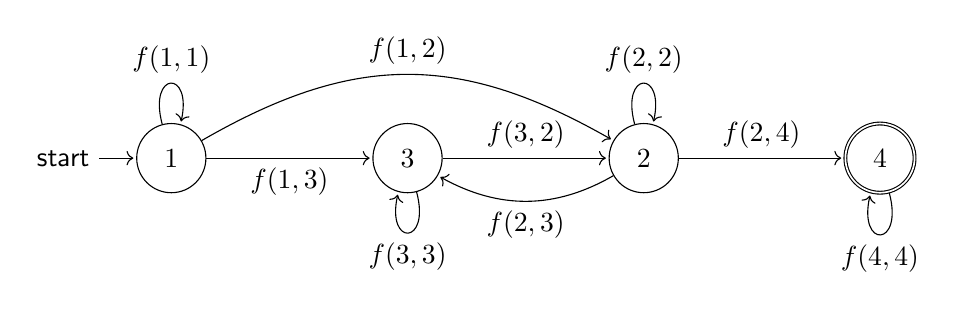
\begin{tikzpicture}[shorten >=1pt, node distance=3cm, on grid, auto]  
				\node[state, initial] (q_0)   {$1$}; 
				\node[state] (q_2) [right=of q_0] {$3$};
				\node[state] (q_1) [right=of q_2] {$2$}; 
				\node[state, accepting] (q_3) [right=of q_1] {$4$}; 
				\path[->]
				(q_0) edge[loop above] node[align=center] {$f(1,1)$} (q_0)
				(q_0) edge node[align=center, below] {$f(1,3)$} (q_2)
				(q_0) edge[bend left, looseness=1.1] node[align=center] {$f(1,2)$} (q_1)
				
				(q_1) edge[loop above] node[align=center] {$f(2,2)$} (q_1)
				edge[bend left, looseness=1.0] node[align=center, below] {$f(2,3)$} (q_2)
				edge node[align=center, above] {$f(2,4)$} (q_3)
				(q_2) edge[loop below] node[align=center] {$f(3,3)$} (q_2)
				edge node[align=center, above] {$f(3,2)$} (q_1)
				(q_3) edge[loop below] node {$f(4,4)$} (q_3); 
			\end{tikzpicture}
        }
        \column{0.52\textwidth}
         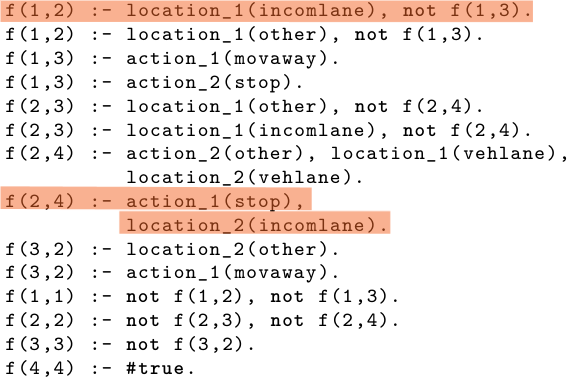
\includegraphics[width=\textwidth]{contents/images/autom_3.png}
    \end{columns}
\end{frame}


\section{NeSy Integration}
{
    \setbeamertemplate{headline}{}
    \begin{frame}
        \sectionpage%
        \begin{tikzpicture}[overlay,remember picture]
            \node[left=2cm] at (current page.2){%
                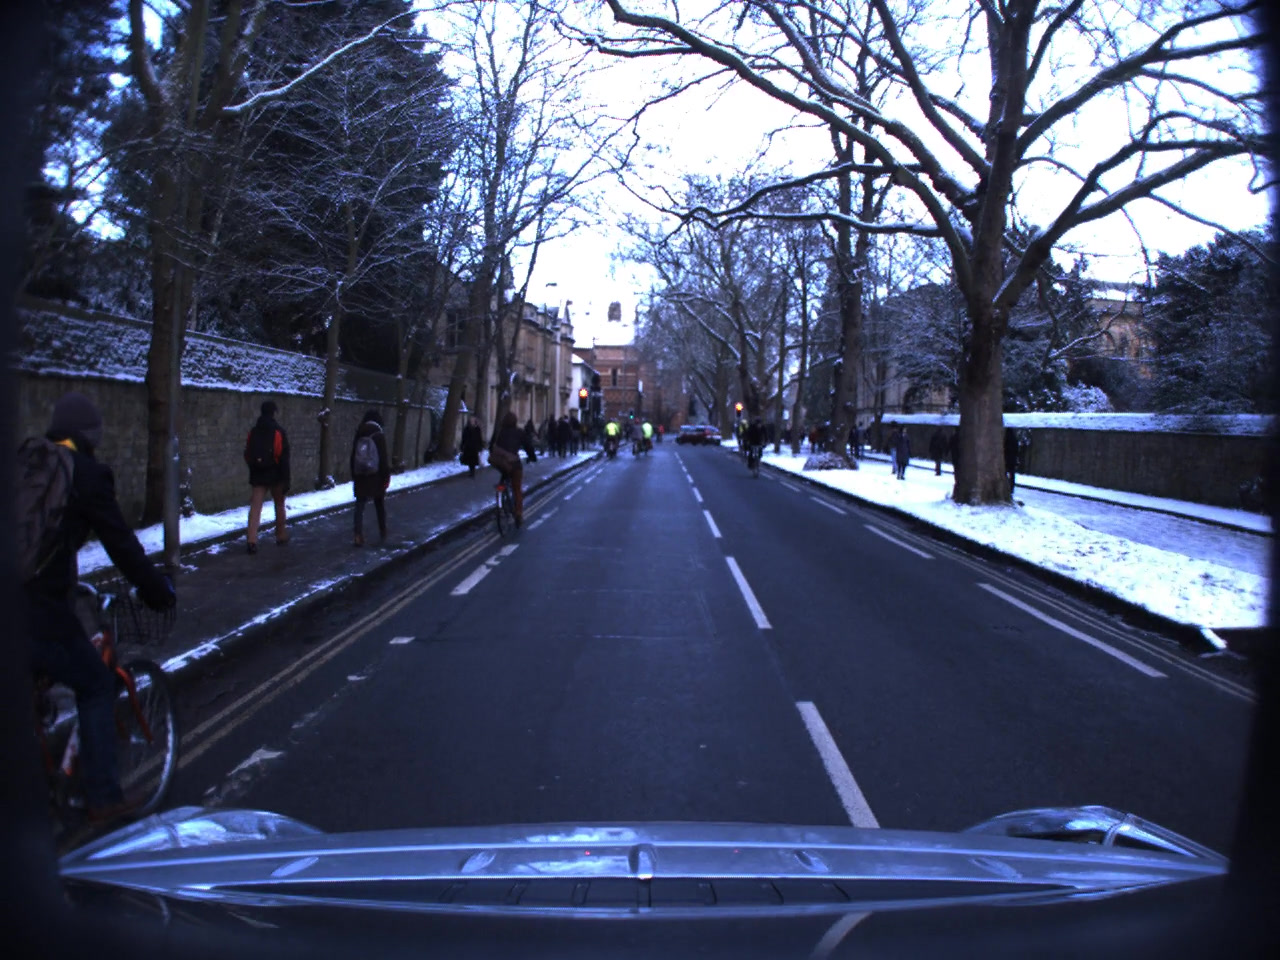
\includegraphics[width=5.5cm]{contents/images/04924}
            };
        \end{tikzpicture}
    \end{frame}
}


\begin{frame}{Neural Component}
 % Networks that will be the neural part of our integration
    \begin{itemize}
        \setlength{\itemsep}{13pt}
        \item A \textbf{single NN} takes as input a \textbf{video} and \colorbf{ bounding boxes of 2 agents} \colorbf{\textit{per frame}}, predicting their \textbf{action} and \textbf{semantic location} (uni-label supervision)
        \item It comprises two modules: \textbf{action recognition} and \textbf{semantic location recognition}
        \item The semantic location recognition module is a simple \textcolor{umBlueLighter}{2D-Convolution} architecture
        \item The action recognition module utilizes both \textcolor{umBlueLighter}{2D} and \textcolor{umBlueLighter}{3D-Convolution} architectures for comparative experiments in NeSy
    \end{itemize}
\end{frame}

\begin{frame}{Probabilistic Inference and Training}
    \begin{figure}
        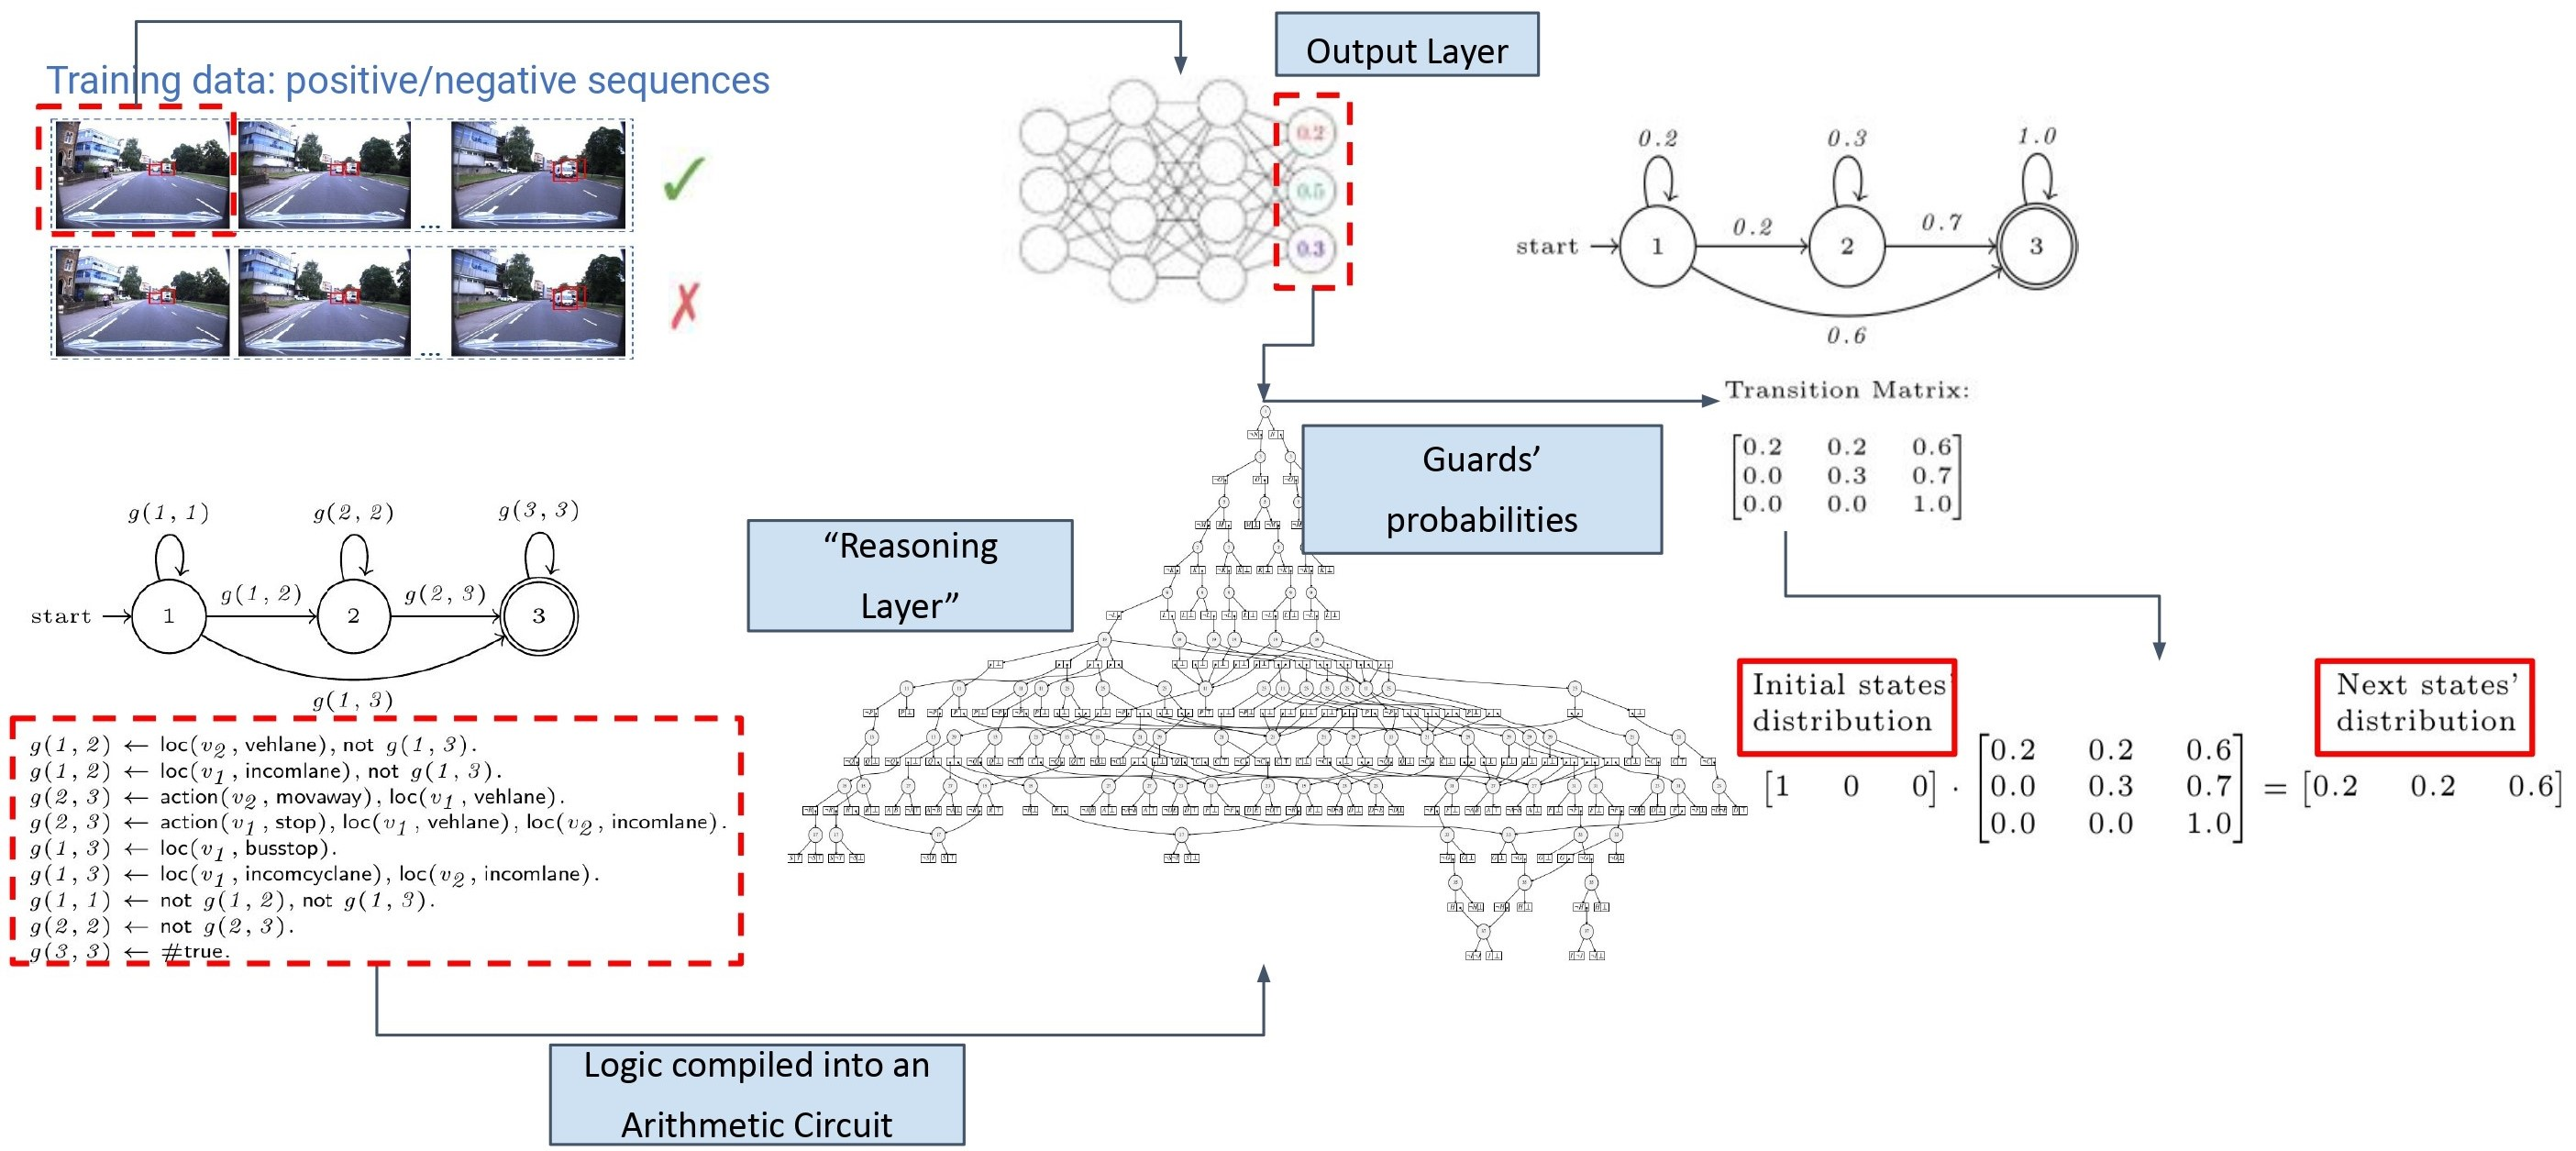
\includegraphics[width=\textwidth]{contents/images/NeSy_training.jpg}
    \end{figure}
\end{frame}


\section{Experiments}
{
    \setbeamertemplate{headline}{}
    \begin{frame}
        \sectionpage%
        \begin{tikzpicture}[overlay,remember picture]
            \node[left=2cm] at (current page.2){%
                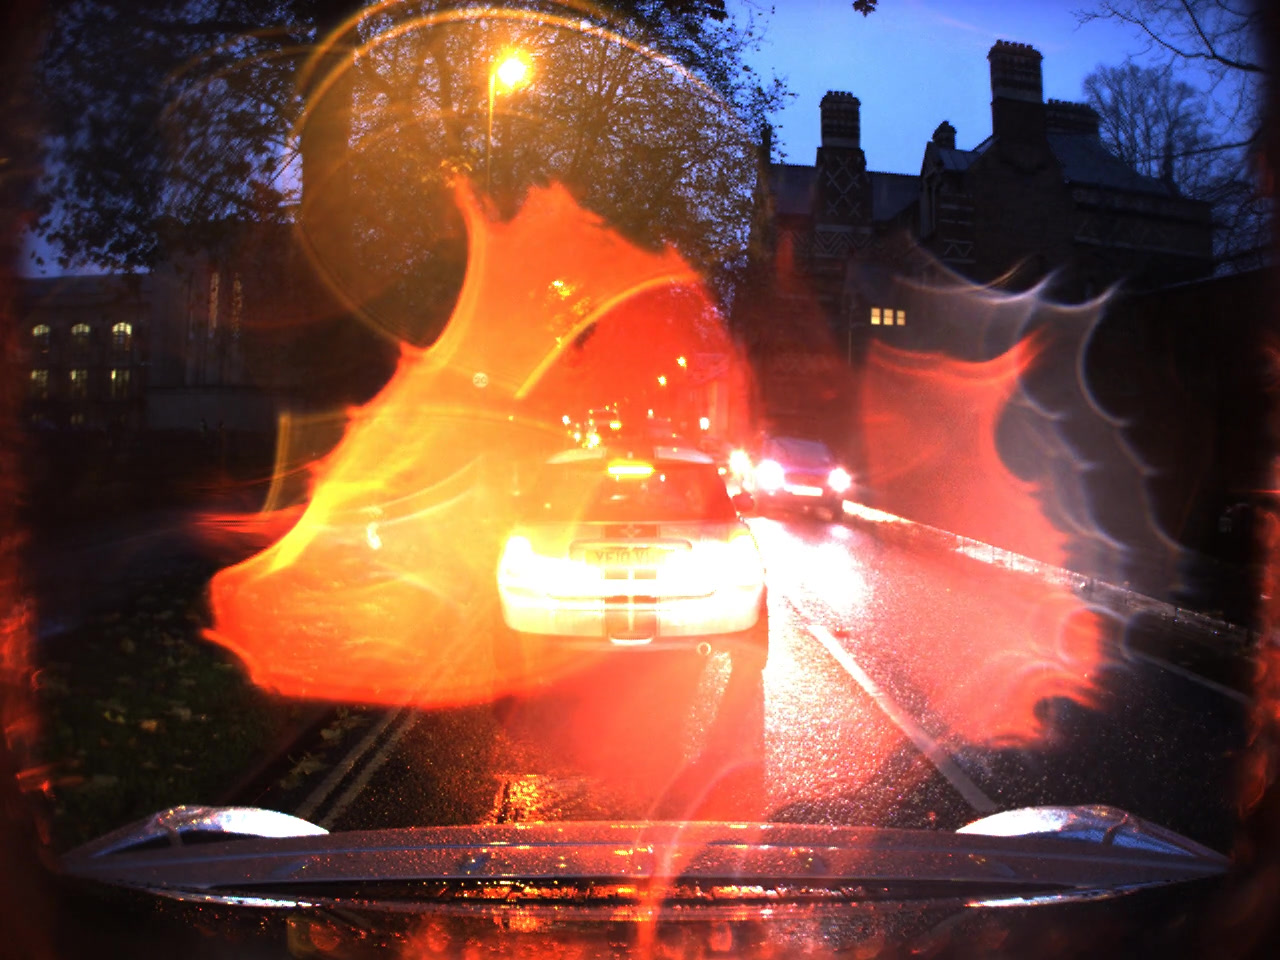
\includegraphics[width=5.5cm]{contents/images/05674}
            };
        \end{tikzpicture}
    \end{frame}
}


\begin{frame}{Experimental Setup}
    \begin{itemize}
    \setlength{\itemsep}{10pt}
    \item \colorbf{Task}: Classify instances as `overtake' incidents or not
    \item Experiments were conducted on \textbf{4 randomly selected data splits}
    \item We evaluated NeSy \textbf{for all 3 automata} against \textcolor{umBlueLighter}{purely neural models}
    \item These models share the same architecture \textit{but} use LSTM for temporal modeling
    \item For action recognition, we used 2D and 3D-CNNs to assess performance across networks with varying trainable parameters
    \item \textbf{Parameter differences}: NeSy has \textit{392,900} [2D-CNN] \& \textit{9,990,000} [3D-CNN]
    \item We also tested different \textbf{loss functions} and methods for handling the NeSy model's \textbf{probability distributions}
\end{itemize}
\end{frame}

\begin{frame}{Loss Functions}
    \begin{itemize}
    \setlength{\itemsep}{12pt}
    \item The dataset is highly \textbf{imbalanced}
    \item We initially used weighted BCE, yielding suboptimal results
    \item We then switched to \colorbf{focal loss}, which down-weights easy examples and emphasizes difficult ones
    \item The NeSy component outputs a \textcolor{umBlueLighter}{probability distribution} over automaton states
    \item We explore two methods:
    \vspace{5pt}
    \begin{itemize}
        \setlength{\itemsep}{3pt}
        \item Utilize only the \textbf{final state probability} as the prediction
        \item Compute the \textbf{Kolmogorov-Smirnov distance} between the state distribution and (0,0,0,1)
    \end{itemize}
    \end{itemize}
\end{frame}

\begin{frame}{Results - Predictions}
    \begin{itemize}
    \setlength{\itemsep}{13pt}
    \item We selected a data split to evaluate the loss function and NeSy probability handling
    \item Evaluations were then conducted on other splits for all automata
    \item The presented evaluation metric is \textbf{F1-micro}
    \end{itemize}
\end{frame}


\begin{frame}{Results - Predictions [Automaton 1]}
\begin{itemize}
    \setlength{\itemsep}{9pt}
    \item Results for the first, \textbf{simple} automaton
    \item Regarding the NeSy model, we configure it using the `State Distribution'
    \end{itemize}
    \begin{table}[H]
	\centering
	\scalebox{0.8}{
		\begin{tabular}{ccc}
			\toprule
			& \cellcolor{umOrange}\textbf{Neural Baseline} & \cellcolor{umBlueLighter}\textbf{NeSy} \\
			\multirow{-2}{*}{\begin{tabular}[c]{@{}l@{}}Data split \\ index\end{tabular}} & \cellcolor{umOrange} F1-micro & \cellcolor{umBlueLighter}F1-micro \\
			\midrule
			\multicolumn{3}{c}{\textit{\textbf{2D}}} \\
			\midrule
			1 & 0.485 & \textbf{0.632} \\
			2 & 0.3 & \textbf{0.649}\\
			3 & 0.446 & \textbf{0.649} \\
			4 & 0.457 & \textbf{0.612}\\
			\midrule
			\multicolumn{3}{c}{\textit{\textbf{3D}}} \\
			\midrule
			1 & 0.549 & \textbf{0.657} \\
			2 & \textbf{0.541} & 0.342 \\
			3 & 0.474 &  \textbf{0.666} \\
			4 & 0.454 & \textbf{0.588}\\
			\bottomrule
		\end{tabular}
	}
\end{table}
\end{frame}

\begin{frame}{Results - Predictions [Automaton 2]}
\begin{itemize}
    \setlength{\itemsep}{9pt}
    \item Results for the second, \textbf{more complex} automaton
    \item Regarding the NeSy model, we configure it using the `State Distribution'
    \end{itemize}
    \begin{table}[H]
	\centering
	\scalebox{0.8}{
		\begin{tabular}{ccc}
			\toprule
			& \cellcolor{umOrange} \textbf{Neural Baseline} &             \cellcolor{umBlueLighter}\textbf{NeSy} \\
			\multirow{-2}{*}{\begin{tabular}[c]{@{}l@{}}Data split \\ index\end{tabular}} & \cellcolor{umOrange}F1-micro & \cellcolor{umBlueLighter}F1-micro \\
			\midrule
			\multicolumn{3}{c}{\textit{\textbf{2D}}} \\
			\midrule
			1 & 0.485 & \textbf{0.597} \\
			2 & 0.3 & \textbf{0.516}\\
			3 & 0.446 & \textbf{0.489} \\
			4 & 0.457 & \textbf{0.582}\\
			\midrule
			\multicolumn{3}{c}{\textit{\textbf{3D}}} \\
			\midrule
			1 & \textbf{0.549} &  0.382\\
			2 & \textbf{0.541} &  0.25 \\
			3 & \textbf{0.474}&   0.326\\
			4 & 0.454 & \textbf{0.538}\\
			\bottomrule
		\end{tabular}
	}
\end{table}
\end{frame}

\begin{frame}{Results - Predictions [Automaton 3]}
\begin{itemize}
    \setlength{\itemsep}{9pt}
    \item Results for the third, \textbf{another complex} automaton
    \item Regarding the NeSy model, 2D $\rightarrow$ `State Distribution' \&  3D $\rightarrow$ `Acceptance Probability'
    \end{itemize}
    \begin{table}[H]
	\centering
	\scalebox{0.8}{
		\begin{tabular}{ccc}
			\toprule
			& \cellcolor{umOrange} \textbf{Neural Baseline} &             \cellcolor{umBlueLighter}\textbf{NeSy} \\
			\multirow{-2}{*}{\begin{tabular}[c]{@{}l@{}}Data split \\ index\end{tabular}} & \cellcolor{umOrange}F1-micro & \cellcolor{umBlueLighter}F1-micro \\
			\midrule
			\multicolumn{3}{c}{\textit{\textbf{2D}}} \\
			\midrule
			1 & 0.567 & \textbf{0.589} \\
			2 & \textbf{0.426} & 0.38 \\
			3 & 0.506 & \textbf{0.613} \\
			4 & 0.331 & \textbf{0.554} \\
			\midrule
			\multicolumn{3}{c}{\textit{\textbf{3D}}} \\
			\midrule
			1 & \textbf{0.684} & 0.63 \\
			2 & 0.437 & \textbf{0.613} \\
			3 & \textbf{0.581} & 0.522 \\
			4 & 0.465 & \textbf{0.549} \\
			\bottomrule
		\end{tabular}
	}
\end{table}
\end{frame}

\begin{frame}{Results - Baseline vs NeSy}
    \colorbf{[Cross-Validation]} :
\begin{table}[H]
	\centering
	\scalebox{1.0}{
		\begin{tabular}{ccccc}
			\toprule
			& \multicolumn{2}{c}{\cellcolor{umOrange}\textbf{Baseline}} & \multicolumn{2}{c}{\cellcolor{umBlueLighter}\textbf{NeSy}} \\
			\multirow{-3}{*}{Automaton} & \cellcolor{umOrange}2D & \cellcolor{umOrange}3D & \cellcolor{umBlueLighter}2D & \cellcolor{umBlueLighter}3D \\
			\midrule
			1 & 0.389 & 0.501 & \textbf{0.637} & \textbf{0.564} \\
			2 & 0.389 & \textbf{0.501} & \textbf{0.542} & 0.391 \\
			3 & 0.439 & 0.53 & \textbf{0.523} & \textbf{0.574}\\
			\bottomrule
		\end{tabular}
	}
\end{table}
\end{frame}

\begin{frame}{Results - NeSy vs Automata}
\begin{table}[H]
	\scalebox{0.95}{
	\begin{tabular}{cccccc}
		\toprule
		& \multicolumn{3}{c}{\cellcolor{umYellow!80}\textbf{Statistics}} & \multicolumn{2}{c}{\cellcolor{umBlueLighter}\textbf{NeSy}} \\
		\multirow{-3}{*}{Automaton} & \cellcolor{umYellow!80}\#transitions & \cellcolor{umYellow!80}avg. literals/transition & \cellcolor{umYellow!80}\#unique simple events & \cellcolor{umBlueLighter}2D & \cellcolor{umBlueLighter}3D \\
		\midrule
		1 & 10 & 1.2 & 4/14 & \textbf{0.637} & \textbf{0.564} \\
		2 & 12 & 1.6 & 7/14 & 0.542 & 0.391 \\
		3 & 14 & 1.6 & 11/12 & 0.523 & 0.574\\
		\bottomrule
	\end{tabular}
	}
\end{table}
\end{frame}

\begin{frame}{Results - Training Evaluation} % many oscillations, loss always less for NeSy
     \begin{minipage}{0.48\textwidth}
        \centering
        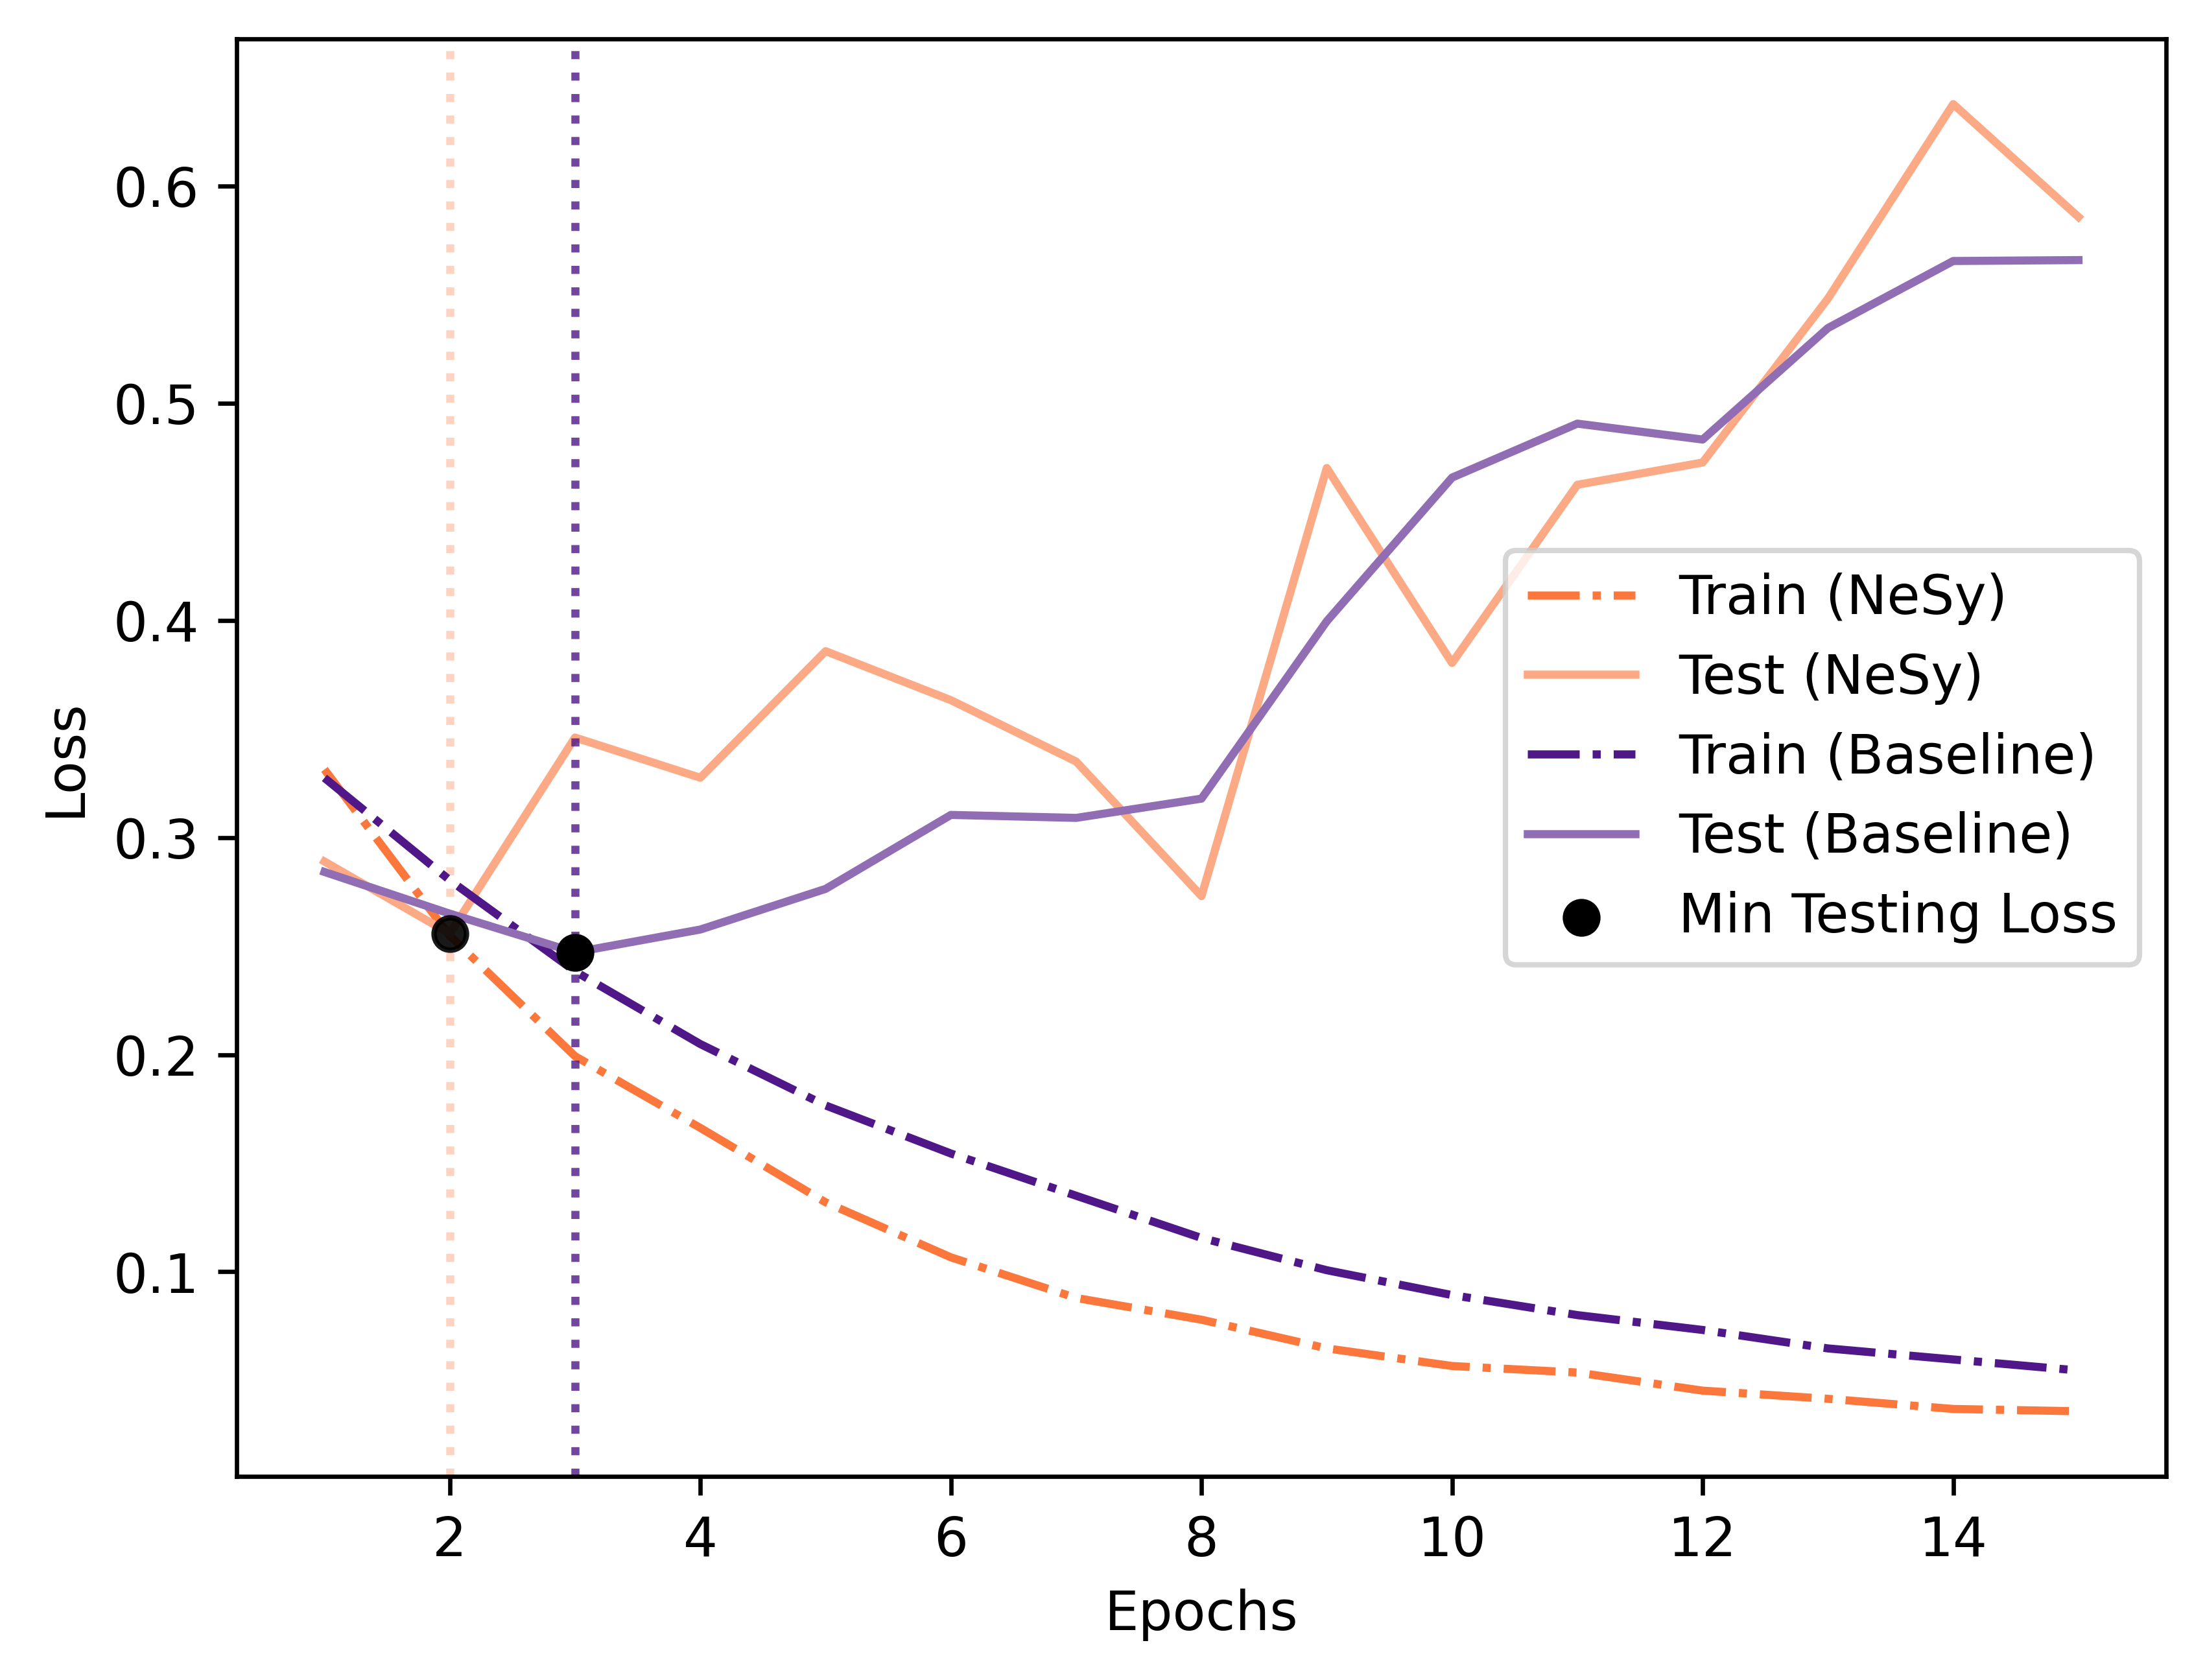
\includegraphics[width=\textwidth]{contents/images/losses_split_14_3d.png}
        \captionof{figure}{Losses}
    \end{minipage}
    \hfill
    \begin{minipage}{0.48\textwidth}
        \centering
        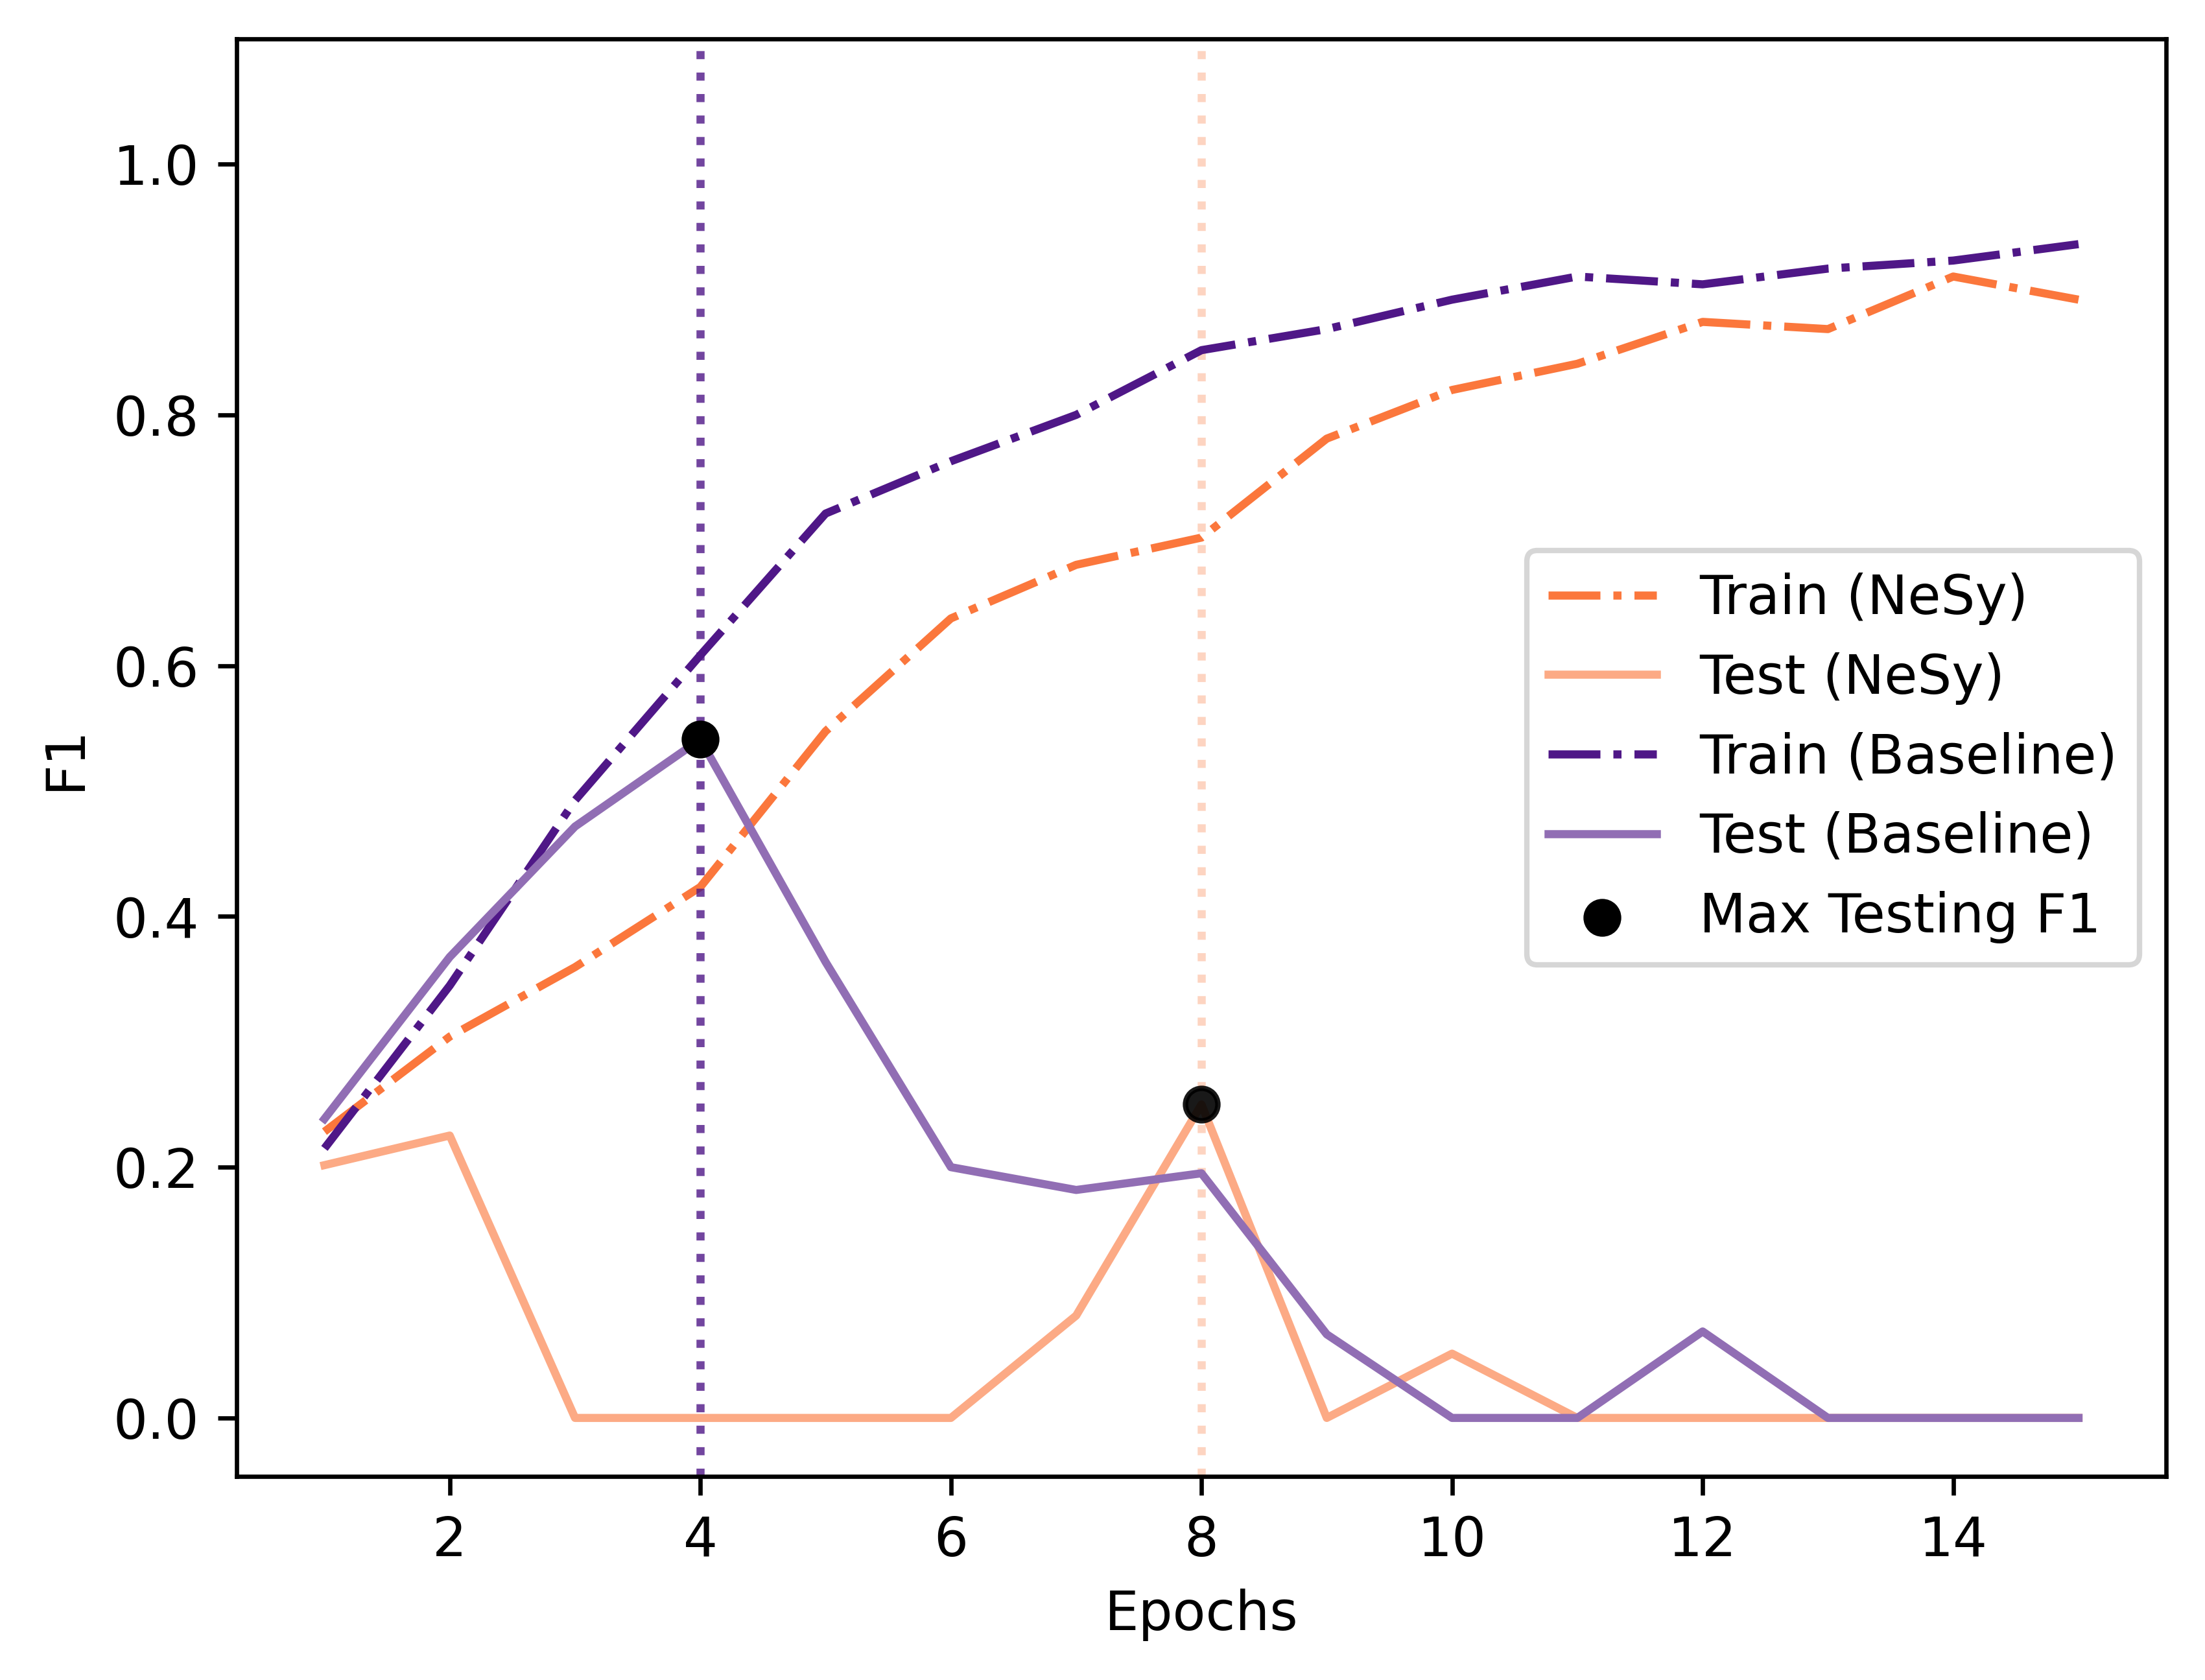
\includegraphics[width=\textwidth]{contents/images/f1_split_14_3d.png}
        \captionof{figure}{Micro-F1}
    \end{minipage}
\end{frame}

\begin{frame}{Results - Training Times / Epoch}
   \begin{table}[H]
	\scalebox{0.95}{
	\begin{tabular}{cccccc}
		\toprule
		& \multicolumn{3}{c}{\cellcolor{umYellow!80}\textbf{Statistics}} & \cellcolor{umOrange}\textbf{Baseline} & \cellcolor{umBlueLighter}\textbf{NeSy} \\
		\multirow{-3}{*}{Automaton} & \cellcolor{umYellow!80}\#trans & \cellcolor{umYellow!80}avg. lit/trans & \cellcolor{umYellow!80}\#unique simple ev. & \cellcolor{umOrange} tt/e & \cellcolor{umBlueLighter} tt/e \\
		\midrule
		1 & 10 & 1.2 & 4/14 & 0.15 sec & \textbf{1.5 mins} \\
		2 & 12 & 1.6 & 7/14 & 0.15 sec & \textbf{4.5 mins} \\
		3 & 14 & 1.6 & 11/12 & 0.15 sec & \textbf{6 mins}\\
		\bottomrule
	\end{tabular}
	}
\end{table}
\end{frame}

\begin{frame}{Results - Simple event training}
   \begin{table}[H]
	\centering
	\scalebox{0.9}{
		\begin{tabular}{p{0.7cm}p{1.6cm}p{1.2cm}p{1.2cm}p{1.6cm}p{1.8cm}p{1.2cm}p{1.2cm}}
			\toprule
			 & \multicolumn{7}{c}{\textbf{Avg. Individual F1-micro}} \\
    \midrule
		&  \cellcolor{umOrange!80}\textbf{movaway} & \cellcolor{umOrange!80}\textbf{stop} & \cellcolor{umOrange!80}\textbf{other} & \cellcolor{umBlueLighter!80}\textbf{vehlane} & \cellcolor{umBlueLighter!80}\textbf{incomlane} & \cellcolor{umBlueLighter!80}\textbf{jun} & \cellcolor{umBlueLighter!80}\textbf{other} \\
			\midrule
			\textbf{2D} & 0.97 & 0.84 & 0.85  & 0.76  & 0.81 & 0.91 & 0.74 \\
			\midrule
			\textbf{3D} & 0.98 & 0.86 & 0.86 & 0.77 & 0.82 & 0.91 & 0.72 \\
			\bottomrule
		\end{tabular}
	}
\end{table}
\end{frame}

\begin{frame}{Results - \textcolor{umBlueLighter}{Simple} to \textcolor{umOrange}{Complex}}
\begin{table}[H]
	\centering
	\scalebox{1.0}{
		\begin{tabular}{l|cc}
			\toprule
			 & \cellcolor{umYellow!70} One-hot encoding & \cellcolor{umYellow!70} Large Probability Mass  (0.8) \\
			\midrule
			 \cellcolor[HTML]{FFFDF6}\textbf{F1-micro} & \textbf{0.947} &  \textbf{0.561}\\
			\bottomrule
		\end{tabular}
	}
\end{table}
\end{frame}


\begin{frame}{Results - \textcolor{umOrange}{Complex} to \textcolor{umBlueLighter}{Simple}}
\begin{table}[H]
	\centering
	\scalebox{0.7}{
		\begin{tabular}{p{1.6cm}p{1.2cm}p{1.2cm}p{1.6cm}p{1.8cm}p{1.2cm}p{1.2cm}}
			\toprule
			 \multicolumn{7}{c}{\textbf{Individual F1-micro}} \\
    \midrule
		\cellcolor{umOrange!80}\textbf{movaway} & \cellcolor{umOrange!80}\textbf{stop} & \cellcolor{umOrange!80}\textbf{other} & \cellcolor{umBlueLighter!80}\textbf{vehlane} & \cellcolor{umBlueLighter!80}\textbf{incomlane} & \cellcolor{umBlueLighter!80}\textbf{jun} & \cellcolor{umBlueLighter!80}\textbf{other} \\
			\midrule
			  0.69 & 0.634 & 0.457 & 0.845 & 0.515 & 0.544 & 0.441\\
			\bottomrule
		\end{tabular}
	}
\end{table}

\vspace{1em}
\colorbf{Reminder}: \textit{When trained on simple events}

\begin{table}[H]
	\centering
	\scalebox{0.7}{
		\begin{tabular}{p{1.6cm}p{1.2cm}p{1.2cm}p{1.6cm}p{1.8cm}p{1.2cm}p{1.2cm}}
			\toprule
			 \multicolumn{7}{c}{\textbf{Avg. Individual F1-micro}} \\
    \midrule
		\cellcolor{umOrange!80}\textbf{movaway} & \cellcolor{umOrange!80}\textbf{stop} & \cellcolor{umOrange!80}\textbf{other} & \cellcolor{umBlueLighter!80}\textbf{vehlane} & \cellcolor{umBlueLighter!80}\textbf{incomlane} & \cellcolor{umBlueLighter!80}\textbf{jun} & \cellcolor{umBlueLighter!80}\textbf{other} \\
			\midrule
			  0.98 & 0.86 & 0.86 & 0.77 & 0.82 & 0.91 & 0.72\\
			\bottomrule
		\end{tabular}
	}
\end{table}
\end{frame}

\section{Conclusions and Future Work}
{
    \setbeamertemplate{headline}{}
    \begin{frame}
        \sectionpage%
    \end{frame}
}

\begin{frame}{Conclusions}
    \begin{itemize}
        \setlength{\itemsep}{13pt}
        \item NeSy has better performance on average
        \item But, undeniably, performs better on \textbf{smaller} models \textit{contrary} to the neural baseline
        \item Its performance and training time depends strongly on the automaton used
        \item Also, it seems to be performing better for more compact automata
        \end{itemize}
    \end{frame}

\begin{frame}{Future Work}
    \begin{itemize}
        \setlength{\itemsep}{13pt}
        \item Try our NeSy method on \textbf{other}, not as imbalanced, datasets
        \item Investigate scalability regarding \textbf{sequence length}
        \item Try other complex event recognition \textbf{architectures}, \textit{e.g., transformers}
        \item More thorough check of the \textbf{relation} between automata and NeSy's performance
        \item Of course, \textbf{joint training}
        \end{itemize}
    \end{frame}


\section{The End}

\begin{frame}
    \begin{center}
        \huge \colorbf{Thank you!} 
        
        Questions?
    \end{center}
    
\end{frame}


\end{document}

